%%%%%%%%%%%%%%%%%%%%%%%%%%%%%%%%%%%%%%%%%%%%%%%%%%%%%%%%%%%%%%%%%%%%%%%%%%%%
%% Author template for Management Science (mnsc) for articles with e-companion (EC)
%% Mirko Janc, Ph.D., INFORMS, mirko.janc@informs.org
%% ver. 0.95, December 2010
%%%%%%%%%%%%%%%%%%%%%%%%%%%%%%%%%%%%%%%%%%%%%%%%%%%%%%%%%%%%%%%%%%%%%%%%%%%%
\documentclass[mnsc,blindrev]{informs3_freeuse} % current default for manuscript submission
%\documentclass[mnsc,nonblindrev]{informs3}

\OneAndAHalfSpacedXI % current default line spacing
%%\OneAndAHalfSpacedXII 
%%\DoubleSpacedXII
%\DoubleSpacedXI

% If hyperref is used, dvi-to-ps driver of choice must be declared as
%   an additional option to the \documentstyle. For example
%\documentclass[dvips,mnsc]{informs3}      % if dvips is used
%\documentclass[dvipsone,mnsc]{informs3}   % if dvipsone is used, etc.

% Private macros here (check that there is no clash with the style)

\usepackage{amsmath,amsfonts,amssymb}
\usepackage{bm}
\usepackage{bbm}
\usepackage{xspace}
\usepackage{color}
%%\usepackage{natbib}
\usepackage[hidelinks,colorlinks,allcolors=black,citecolor=magenta]{hyperref}
\let\oldciteauthor=\citeauthor
\def\citeauthor#1{\hypersetup{citecolor=black}\oldciteauthor{#1}}
\usepackage{wrapfig}
\usepackage{anyfontsize}
\usepackage{subcaption}
\usepackage{cleveref}
\usepackage{tikz,pgfplots}
\usepackage{algpseudocode,algorithm}
\pgfplotsset{compat=1.11}
%\addtolength{\oddsidemargin}{-.9in}
%        \addtolength{\evensidemargin}{-.9in}
%        \addtolength{\textwidth}{1.25in}
%        \addtolength{\topmargin}{-.55in}
%        \addtolength{\textheight}{1.5in}

\usepackage{multicol}
\usepackage{array}
\newcolumntype{M}[1]{>{\centering\arraybackslash}m{#1}}

\usepackage{tikz}
\usetikzlibrary{arrows,matrix,positioning,fit}
\usepackage{nicefrac}
\usepackage{thmtools,thm-restate}
\usepackage[arrowdel]{physics}

\usepackage{pifont}
\newcommand{\cmark}{\ding{51}\xspace}%
\newcommand{\xmark}{\ding{55}\xspace}%

\newcommand*\circled[1]{\tikz[baseline=(char.base)]{%
		\node[shape=circle,draw,inner sep=2pt] (char) {#1};}}

% \newtheorem{proposition}{Proposition}
% \newtheorem{corollary}{Corollary}
% \newtheorem{theorem}{Theorem}
% \newtheorem{lemma}{Lemma}
% \newtheorem{conjecture}{Conjecture}
% \newtheorem{question}{Question}
% \theoremstyle{definition}
% \newtheorem{definition}{Definition}
%\newtheorem{example}{Example}
% \newtheorem{examplex}{Example}
% \newenvironment{example}{\pushQED{\qed}\examplex}{\popQED\endexamplex}

%\renewcommand{\cite}{\citep}

%\usepackage{xcolor}
%\usepackage{color,soul}
%\usepackage{amsmath}
%\usepackage{amssymb}
%\usepackage{mathtools}
%\usepackage{cleveref}
\usepackage{longtable}
\usepackage{makecell}
\usepackage{subcaption}

\newcount\Comments  % 0 suppresses notes to selves in text
\Comments=1
\newcommand{\kibitz}[2]{\ifnum\Comments=1{\color{#1}{#2}}\fi}
\newcommand{\rf}[1]{\kibitz{blue}{[Roy says:#1]}}
\newcommand{\kg}[1]{\kibitz{brown}{[Kobi says:#1]}}
\newcommand{\gb}[1]{\kibitz{red}{[GB:#1]}}
 
\newcommand{\points}{\textsc{Points}}
\renewcommand{\rank}{\textsc{Rank}}
\newcommand{\vfm}{\textsc{Vfm}}
\newcommand{\knap}{\textsc{Knap}}
\newcommand{\kapp}{\textsc{Kapp}}
\newcommand{\tapp}{\textsc{Tapp}}
\newcommand{\sw}{\textsc{sw}}
\newcommand{\voters}{{N}}
\newcommand{\mes}{ES}
\newcommand{\pabu}{PaBuLib}
\newcommand{\costes}{\textsc{ES-C}}
\newcommand{\costgreedy}{\textsc{Greedy-C}}
\newcommand{\bines}{\textsc{ES-B}}
\newcommand{\bingreedy}{\textsc{Greedy-B}}

%----------------------------------------

\usepackage{mathtools}

\usepackage{booktabs} % For formal tables

% Natbib setup for author-year style
\usepackage{natbib}
 \bibpunct[, ]{(}{)}{,}{a}{}{,}%
 \def\bibfont{\small}%
 \def\bibsep{\smallskipamount}%
 \def\bibhang{24pt}%
 \def\newblock{\ }%
 \def\BIBand{and}%

%% Setup of theorem styles. Outcomment only one. 
%% Preferred default is the first option.
\TheoremsNumberedThrough     % Preferred (Theorem 1, Lemma 1, Theorem 2)
%\TheoremsNumberedByChapter  % (Theorem 1.1, Lema 1.1, Theorem 1.2)
\ECRepeatTheorems

%% Setup of the equation numbering system. Outcomment only one.
%% Preferred default is the first option.
\EquationsNumberedThrough    % Default: (1), (2), ...
%\EquationsNumberedBySection % (1.1), (1.2), ...

% In the reviewing and copyediting stage enter the manuscript number.
%\MANUSCRIPTNO{} % When the article is logged in and DOI assigned to it,
                 %   this manuscript number is no longer necessary

%%%%%%%%%%%%%%%%
\begin{document}
%%%%%%%%%%%%%%%%

% Outcomment only when entries are known. Otherwise leave as is and
%   default values will be used.
%\setcounter{page}{1}
%\VOLUME{00}%
%\NO{0}%
%\MONTH{Xxxxx}% (month or a similar seasonal id)
%\YEAR{0000}% e.g., 2005
%\FIRSTPAGE{000}%
%\LASTPAGE{000}%
%\SHORTYEAR{00}% shortened year (two-digit)
%\ISSUE{0000} %
%\LONGFIRSTPAGE{0001} %
%\DOI{10.1287/xxxx.0000.0000}%

% Author's names for the running heads
% Sample depending on the number of authors;
% \RUNAUTHOR{Jones}
% \RUNAUTHOR{Jones and Wilson}
% \RUNAUTHOR{Jones, Miller, and Wilson}
% \RUNAUTHOR{Jones et al.} % for four or more authors
% Enter authors following the given pattern:
%\RUNAUTHOR{Freeman et al.} %Commented this out for submission since it was generating "Freeman et al." as a header on e-companion pages

% Title or shortened title suitable for running heads. Sample:
% \RUNTITLE{Bundling Information Goods of Decreasing Value}
% Enter the (shortened) title:
\RUNTITLE{Participatory Budgeting  Designs for the Real World}

% Full title. Sample:
% \TITLE{Bundling Information Goods of Decreasing Value}
% Enter the full title:
\TITLE{Participatory Budgeting  Designs for the Real World\footnote{A preliminary version of this paper appeared at AAAI 2023.}}

% Block of authors and their affiliations starts here:
% NOTE: Authors with same affiliation, if the order of authors allows,
%   should be entered in ONE field, separated by a comma.
%   \EMAIL field can be repeated if more than one author
\ARTICLEAUTHORS{%
\AUTHOR{Roy Fairstein}
\AFF{Ben-Gurion University of the Negev, Israel, \EMAIL{royfa@post.bgu.ac.il}} %, \URL{}}
\AUTHOR{Gerdus Benad\`{e}}
\AFF{Boston University, MA, USA, \EMAIL{benade@bu.edu}}
\AUTHOR{Kobi Gal}
\AFF{University of Edinburgh, UK}
\AFF{Ben-Gurion University of the Negev, Israel  \EMAIL{kobig@bgu.ac.il}} 
% Enter all authors
} % end of the block

%\title{Participatory Budgeting  Designs for the Real World}

% \author{\name Roy Fairstein \email royfa@post.bgu.ac.il \\
%        \addr  Ben-Gurion University of the Negev, Israel
%        \AND
%        \name Gerdus Benad\`{e} \email benade@bu.edu \\
%        \addr Boston University, MA, USA
%        \AND
%        \name Kobi Gal \email kobig@bgu.ac.il \\
%        \addr Ben-Gurion University of the Negev, Israel \\
%        University of Edinburgh, UK }

\ABSTRACT{ 
Participatory budgeting (PB) is a type of crowdfunding which engages the inhabitants of a city  in the process of allocating  public money to different types of projects. 
PB elections often suffer from extremely low voter turnout, highlighting the need to design   elections   that   are accessible to voters from all socio-economic backgrounds. 
 % PB processes  differ in how voters are asked to express their preferences over candidate projects and how these preferences are aggregated to determine which projects to fund. 
  %This paper studies  the fundamental questions  of PB design: what voting format and aggregation method should you use?
  This paper studies six voting formats and two prominent aggregation methods towards answering the fundamental questions  of PB design: how should voter express their preferences over candidate projects, and how should those preference be aggregated  to determine which projects to fund?
  We conduct an   experiment in which $1\,800$ participants vote in four participatory budgeting elections  to evaluate the practical effects of these design decisions. % the choice of voting format and aggregation rule. 
    Among voting formats, we find  that $k$-approval voting leads to the best voter experience. 
    We find little separation between the leading aggregation rules in terms of welfare and representation. 
    %In terms of stability, or the robustness of the rule to the choice of input format and partial participation, 
    The method of equal shares is much more stable, or robust to the choice of input format and partial participation, than greedy aggregation.
    %With respect to the aggregation rule, we focus on stability, or the robustness of the rule to the choice of input format and partial participation. Greedy aggregation leads to outcomes that are  highly sensitive to   the input format used and the fraction of the population that participates. The method of equal shares, in contrast, leads to outcomes that are not sensitive to the type of voting format used, and these outcomes are remarkably stable even when the majority of the population does not participate in the election.  
    The findings from our user study are  replicated on data from a repository of 532 real participatory budgeting elections. }

% Fill in data. If unknown, outcomment the field
\KEYWORDS{...} 
%\HISTORY{This paper was first submitted on April 12, 1922 and has been with the authors for 83 years for 65 revisions.}


 


\maketitle



%\cite\

\section{Introduction}\label{sec:intro}
%alternative
% PB process + spreading, cool and exciting
% but it faces some challenges - low participation
% in light of this, design is important, balance many factors. Elicitation + aggregation
% Elicitation + discussion
% aggregation + discussion

Participatory budgeting (PB) is an exciting form of direct democracy that allows a community to take part in deciding how to allocate a budget among different projects.  
A participatory budgeting election  consists of several phases. First, organizers elicit proposals for  projects. These proposals are developed further (expanded, merged, costed, etc.) and finally filtered to a set of candidate projects.  Citizens are then asked to cast a vote which expresses a preference over the candidate projects, and the votes are aggregated to determine which projects are funded.
%

Participatory budgeting was introduced in Porto Alegre in Brazil in an attempt to increase transparency of the local government. Since then it has grown in  popularity around the world for many of the same reasons the broader crowdfunding movement is popular: It leads to creative solutions to   problems, helps connect and empower communities with shared interests,  and increases engagement and ownership around local policies.
Today, participatory budgeting elections have been held in many major cities including Madrid, Rome, Paris and New York~\citep{sintomer2008participatory,su2017porto}.  %One benefit of participatory budgeting is that it can increase community satisfaction by allowing voters to affect local decisions that matter to them. 

%Like most democratic innovations, participatory budgeting also faces very real challenges. 
Despite  its increasing adoption over the last two decades, participatory budgeting also faces  unique challenges. 
For example, participation rates in PB elections can be low, in  extreme cases as low as 0.1\% in Germany~\citep{zepic2017participatory} and 1-3\%   in Chicago in 2012 and 2014~\citep{stewart2014participatory,carroll2016democratizing}. In traditional crowdfunding settings engagement is a signal of market interest, and low participation may imply that a proposed product does not have a large audience.   
In participatory budgeting, however, the effect of low   participation is that a small group of voters   determines how to allocate a potentially large pool of public funds that was intended to benefit the entire community. This can easily create or reinforce social inequalities. 
% in traditional crowdfunding settings, low participation simply indicates that the products/services dont have a market
%here in contrast, the effect is that a small group of voters determines the allocation of a pool of funds intended to benefit the entire community. potentially causing or perpetuation social inequalities. 

% ---
% Participatory budgeting (PB) is an exciting form of direct democracy that allows a community to take part in deciding how to allocate a budget among different projects. 
% %It is growing in popularity and has been used around the world including in major cities like Madrid, Rome, Paris~\citep{sintomer2008participatory} and New York~\citep{su2017porto}.  One benefit of participatory budgeting is that it can increase community satisfaction by allowing voters to affect local decisions that matter to them. 
% %allows voters to affect local policies that matter to them, and  can increase community satisfaction when  better sets of projects are funded. 
% %
% A participatory budgeting election  consists of several phases. First, organizers elicit proposals for  projects. These proposals are developed further (expanded, merged, costed, etc.) and finally filtered to a set of candidate projects.  Citizens are then asked to cast a vote which expresses a preference over the candidate projects, and the votes are aggregated to determine which projects are funded.
% %
% Participatory budgeting is growing in popularity around the world, in part because it empowers communities to have a direct say on local policies that affect them,  and it has been used  in major cities like Madrid, Rome, Paris and New York~\citep{sintomer2008participatory,su2017porto}.  %One benefit of participatory budgeting is that it can increase community satisfaction by allowing voters to affect local decisions that matter to them. 

% %Like most democratic innovations, participatory budgeting also faces very real challenges. 
% Despite the early success of participatory budgeting and its increasing adoption over the last two decades, it also faces very real challenges. 
% For example, participation rates in PB elections are often low, in  extreme cases as low as 0.1\% in Germany~\citep{zepic2017participatory} and 1-3\%   in Chicago in 2012 and 2014~\citep{stewart2014participatory,carroll2016democratizing}. 
% % in traditional crowdfunding settings, low participation simply indicates that the products/services dont have a market
% %here in contrast, the effect is that a small group of voters determines the allocation of a pool of funds intended to benefit the entire community. potentially causing or perpetuation social inequalities. 

% ---

We study the complex task of  designing  participatory budgeting elections that are inclusive, easy to participate in, and produce high quality outcomes.   In particular, we assume that a shortlist of candidate projects have been fixed through some process and focus on the latter two components of the election: \emph{preference elicitation} ---  how voters are asked to express their preferences, and \emph{aggregation} --- how votes are aggregated to determine which projects to fund. 


In terms of preference elicitation,   voters should be able to express complex preferences over projects, for example, a voter may   prefer exactly one library being built rather than zero or two, while being indifferent between the two proposed locations. At the same time, voting should be accessible to everyone  no matter their educational or socio-economic background, and there is a real risk that requiring too much information from voters can deter   participation. 
Very simple voting formats   come with their own problems and can lead to frustration and disillusionment. 
Organising bodies  may also have secondary objectives, for example, designing an input format which exposes voters to   budgetary constraints similar to what the city council faces.  
%

The vast majority of real-world PB elections use $k$-approval voting \citep{aziz2021participatory}, in which a voter approves their most preferred $k$ projects, though we are we aware of little formal justification for this choice.  Other formats that have been proposed in the literature or used in practice include knapsack voting (voters approve their most preferred budget-feasible set)  \citep{goel2019knapsack}, ranking projects by value or value-for-money  \citep{aziz2020expanding,benade2021preference} and reporting (typically additive)  utilities \citep{peters2021proportional}. 

When it comes to aggregation,  the funded projects should   reflect the preferences of  as large a part of the population as possible. Outcomes are commonly evaluated in terms of \emph{social welfare}, using some proxy for voter utility functions derived from their votes, and \emph{representation}, which tries to capture whether the preferences of every subgroup in the population (for example, each neighbourhood) contributed to the outcome in proportion  to the subgroup's size. We propose two new axes on which to evaluate aggregation methods: \emph{stability to partial participation} and \emph{responsiveness to campaigning}. 
%
First, in light of low real-world turnout at participatory budgeting elections, we posit that  a desirably property of an aggregation rule is a form of \emph{stability}, or robustness. 
We distinguish between two forms of stability. In the first, the outcome of the election is robust to the choice of input format --- this allows the organizers to freely select an input format without fear of affecting the outcome of the election. In the second, the outcome of the election is robust to partial participation --- voter turnout may be low in real PB elections, ideally the outcome of the election is not drastically affected by the {(non-)participation} of a potentially sizable random   group of   voters. 
%
Second, we study the extent to which different elections are responsive to campaigning, which may be regarded as a form of strategic behaviour. In the time between    the announcement of the project set and the actual voting process, various groups may engage in campaigns aimed at persuading others to vote for specific project sets, as exemplified by the case in Poland in 2015~\citep{polko2015models}. Campaigning, in and of itself, is not inherently good or bad. It can be a form of grassroots engagement, but it may also open the door for corporations or wealthy individuals to sway elections towards their interests. 
Understanding of the effect of aggregation rule on the sensitivity of the election to campaigning will help organizers make informed decisions to mitigate or amplify the effects of such campaigns and allow individuals to assess the potential benefits of participating in campaigns.

%Another aspect of participatory budgeting (PB) that has received limited attention in the existing literature pertains to the utilization of campaigning, which can be regarded as a form of strategic behavior. In such scenarios, during the interval between the publication of the project set and the actual voting process, various groups may engage in campaigns aimed at persuading others to vote for specific project sets, as exemplified by the case in Poland in 2015~\citep{polko2015models}. This study focuses on examining the responsiveness of aggregation rules to changes in votes, thereby elucidating the sensitivity of these rules to campaigning activities. A comprehensive understanding of this dynamic would aid organizers in making informed decisions to mitigate or amplify the impact of such campaigns on the overall outcome according to their objectives. Additionally, it would empower individuals to assess the potential benefits they could derive from participating in these campaigns, enabling them to determine whether their efforts are worthwhile.

Real-world elections almost exclusively use some form of greedy aggregation in which projects are selected in decreasing order of the number of approvals   received. The Method of Equal Shares (\mes{})~\citep{peters2021proportional}, which was used in elections in Switzerland and Poland in 2023,  is perhaps the only real challenger to greedy aggregation.
Alternatives like Cumulative Single Transferable Vote~\citep{skowron2020participatory} and variations on the greedy approach~\citep{talmon2019framework}   are yet to be of practical significance.



We perform   a comprehensive  study of the effect of voting format and aggregation rule on  both the voter experience and the quality of the resulting outcomes    towards answering the fundamental design question of
\emph{what input format and aggregation method should be used  in participatory budgeting elections?
}

\subsection{Our Contributions}

%corporate fundraising  - GOrd


Our study consists of two types of datasets: a user experiment    with more than $1\,800$ participants, and a computational study on publicly available data from 532  real participatory budgeting elections. This data is used in two parts: comparing different input formats (ways to elicit the preferences) to understand which of them is the best to use, and aggregation methods comparison to understand their properties and which of them should be used.

% Our study consists of two parts: a user experiment    with more than $1\,800$ participants, and a computational study on publicly available data from 532  real participatory budgeting elections. 

At the first part, we utilize the data acquired during the experiment to test the different input format. Subsequently, in the second part we conduct a comparative analysis between the outcomes achieved by employing both greedy aggregation and \mes{} on the cast votes.  Throughout our evaluation we use the most common ways of associating votes with utilities from the literature: either binary (\{0,1\}) or cost (\{0, cost\}) utilities.
When we undertake a comparison between two utility formats, we assume that we are referring to the same aggregation method. Conversely, when we compare aggregation methods, we assume a consistent utility format for the evaluation.


% \gb{we user experience on mturk to compare input formats, on both ...} We compare the outcomes from using greedy aggregation and \mes{} on the votes cast.  Throughout our evaluation we use the most common ways of associating votes with utilities from the literature: either binary (\{0,1\}) or cost (\{0, cost\}) utilities.
% When we compare two utilities format we assume that we talk about the same aggregation method and the other way, when comparing aggregation method, we assume the same utility format.\gb{something like this}

We recruit more than $1\,800$ participants on Amazon Mechanical Turk (MTurk),  present each with one of four different PB elections  and ask them to vote in one of six   input formats. 
We track several aspects of the voter experience, including the time it takes to learn and use each format and voters' self-reported belief that an input format accurately captures their preferences.  
%
We find that $k$-approval voting leads to the best voter experience. Voters using $k$-approval spent the least time  learning the format and casting their votes and found the format easiest to use. Somewhat surprisingly, voters also felt that  it was the format that allowed them to express their preferences best, despite the fact that $k$-approval captures strictly less information about voter preferences than, for example,  a ranking of the projects. 


When comparing the aggregation methods, we find no significant difference in   social welfare and representation of these rules.  
We define a new notion of entropy to measure stability and 
mimic partial participation by repeatedly sampling a small fraction of the  votes cast in each election, aggregating the sample and tracking the outcome. %\footnote{We also attempt to compare the social welfare of the outcomes from different aggregation methods and don't find significant differences. Refer to the appendix for further details. }  %Although the two methods lead to comparable social welfare, we identify two  advantages of \mes{} over greedy aggregation.
We find that binary utilities has two advantages over cost utilities on this axis. 
First, it is much less sensitive to the input format used --- no matter the input format used, the set of projects that are funded remains almost identical. This makes the aggregation very versatile: as long as it is used for aggregation, the designer can choose almost any reasonable input format to satisfy whatever secondary objectives are present without fear that this will distort the outcome of the election. 
Second, we find that using binary utilities make the aggregation remarkably stable as participation decreases. In fact, sampling as few as 25-50\%  
of the voters and aggregating only the sampled votes rarely leads to a change in the set of projects being funded. 
Furthermore, we demonstrate that employing \mes{} instead of the greedy approach leads to more robust outcomes. The degree of robustness observed is contingent upon the specific selection of utilities.
% \gb{new sentence: across utilities, es still more stable than greedy}
In light of low levels of real-world participation, we believe this is a particularly attractive property (and one  not shared by greedy aggregation). 
Finally, we find that stability is inversely correlated with responsiveness.

% Further, we find that stability is inversely correlated with responsiveness: greedy aggregation is consistently more responsive to campaigning than \mes. \gb{for the same utility format}%, though voters see benefits from campaigning after swaying roughly 5\% of the voting population under both aggregation methods. 
% \rf{We need to be more careful over here as the results you described are not necessarily correct. greedy is more responsive than ES for pabulib, but this is not the case for the study (which seems the paragraph talk about). Also, I'm not sure where you brought the number 5\% from, we require a minimum of 11.5\% for the study and more for pabulib}\rf{It might worse mentioning here or on the pabulib paragraph that the responsiveness results for the study don't show significant change, i.e. expect greedy-C, they all have value of 0.217-0.28, and since there are 40~60 voters, the difference in number of voters is just a couple voters.} \gb{removed the number 5 (did a plot change?) greedy being more responsive  is straight from   fig 10.}\gb{how do you want to write this?}
\gb{}


Next, we investigate whether our findings  can be replicated outside the confines of our user experiment. We use publicly available data from \pabu{} from 523 real-world participatory elections. These elections have up to 89,000 voters and 137 projects, and voters cast approval votes.  
On small instances with less than 10 projects and those that are tightly constrained, in the sense that at most two randomly selected projects can be funded, there is little difference in stability between \mes{} and greedy aggregation. However, on larger instances where there is more flexibility and a greater number of feasible outcomes, \mes{} is consistently and significantly more stable than greedy aggregation. As before, greedy aggregation proves 
 to be more responsive to campaigning.  
 The findings of our study indicate that \mes{} exhibits greater stability compared to the greedy aggregation method, when considering the same utility format, while here we observe consistent stability superiority of \mes{} over greedy aggregation, regardless of the specific choice of utilities.
 We posit that this disparity arises from the size of the instances considered. The study encompassed instances with $40\sim60$ voters, while pabulib comprises instances with significantly larger voter populations, with some instances containing hundreds, many with thousands, and even tens of thousands of voters. Consequently, in the study with smaller instances, even minor changes in the votes can exert a notable impact on the results. However, in the context of the pabulib dataset, much more substantial changes in the votes are necessary to produce a similar effect on the outcomes. This discrepancy in voter population size thus contributes to the observed differences in stability between the two scenarios.
 % These findings do not depend on the choice of utility model and are consistent with what we found in the user study. 

Our study provides a structured comparison of participatory budgeting design choices with valuable insights for   practitioners. 
Compared to current practice of using $k$-approval votes and greedy aggregation we find evidence for the continued use of $k$-approval and against greedy aggregation. Voters find $k$-approval easy of use and expressive, while greedy aggregation is unstable in  the face of partial participation and more susceptible to having the outcome swayed by campaigning. 
The data set collected during the user experiment is publicly available; we  hope that it will benefit future research.  % Our dataset and code will be made publicly available. 
 
 
\section{Related Work }\label{sec:related}
%ibm stuff, homebias in crowd funding



Participatory budgeting has received a lot of attention from the artificial intelligence and optimization communities over the last 7 years;  see \citet{aziz2021participatory}  for a thorough review.

Our work is closest to two studies that report on user experiments. In the first,  \citet{benade2018efficiency}  study the role of input formats in lab controlled PB settings. They ask participants  to express preference over items that may aid their survival in a desert island. Each item has a weight and participants are informed that they can only carry items up to a specified weight limit. 
\citet{benade2018efficiency} report on the time it takes to vote, the consistency of preferences across format, and the average and worst-case welfare  of different aggregation methods. % (under the assumption that the utility of an alternative is equal to the points assigned to it).
In their work, voters face only a single set of alternatives (election), and the desert island framing is far removed from PB as practiced in cities.  It is unlikely that their findings are general  (for example, there may be an obvious budget-feasible set of alternatives that best aids survival).   Our experiment   mimics real-world participatory budgeting elections much more closely by using projects from real elections and  locating projects and voters on a city map. We   validate our findings by repeating the experiment across four elections with different sizes and projects. 
In the second study, 
\citet{goel2019knapsack} propose knapsack votes and empirically compare       value-for-money comparisons, knapsack and $k$-approval votes in several ways, including through a user survey. It is found that knapsack and $k$-approval votes take a similar amount of time, while value-for-money comparisons impose less cognitive load.  We find the opposite: voters consistently take significantly longer to  form value-for-money rankings. One possible explanation is that \citet{goel2019knapsack} performed a pair-wise comparison between projects, while we ask the voters for a full ranking over all projects. %\citet{goel2019knapsack}   show some theoretical properties of knapsack under overlap utilities. 

On the theory side, 
\citet{benade2021preference}  study the   information content of different input formats in a worst-case model.
They also conduct simulations, using votes from real PB elections,  to evaluate the social welfare that result from different input formats under a particular aggregation rule. They find that `threshold approval' have both the strongest theoretical guarantees and highest welfare in simulations. Threshold approval does not stand out in our results. \citet{MPSW19} extend this idea to measure the optimal tradeoff between the number of bits a vote requires and the resulting worst-case welfare guarantees.

A large literature studies the axiomatic properties of aggregation rules. Analysis most often focuses on maximizing the social welfare of the outcome \citep{benade2021preference,goel2019knapsack,jain2020participatory,hershkowitz2021district,talmon2019framework} %\gb{other papers that maximize welfare?} 
or satisfying some version of proportionality, which (roughly) requires that a group of voters  with similar opinions should have impact on the outcome proportional to the size of the group \citep{fain2016core,aziz2017justified,sanchez2017proportional,fain2018fair,aziz2018proportionally,skowron2020participatory,peters2021proportional} or both \citep{fairstein2022welfare,michorzewski2020price}.  Notably, \mes{} satisfies a proportionality condition called extended justified representation that guarantees a degree of representation to minority groups with common interests \citep{PS20}. 

%In addition to  welfare and representation we evaluate  the stability of greedy aggregation and \mes{}, which  concerns the degree to which the outcome changes as one varies either the input format used in the election, or the degree of participation.  
To the best of our knowledge stability, which  concerns the extent to which the election outcome changes as one varies either the input format   or degree of participation,    has not been studied before. 
What we call \emph{responsiveness to campaigning}  is   related to   the manipulability of elections \citep{Gib73,Sat75,BTT89}. In a classical variant of the single-winner election manipulation problem one asks if a voter (or  coalition of voters) can, keeping the remainder of the instance fixed,  cast their votes to strategically to cause a specific candidate to win. We measure the responsiveness of an aggregation rule by the average number of identical voters that a randomly selected voter must  persuade to yield a better outcome  according to the preferences of this voter.  
The (in)ability of an individual voter to influence the outcome of an election reminds of the expressive theory of voting \citep{brennan1984voter}   under which voting is, according to \cite{brennan1997democracy},  an ``action that is
undertaken for its own sake rather than to bring about particular consequences.''
More responsive aggregation rules prevent this form of voter disillusionment, however, they also open the door for whoever is able to afford an extensive campaign to sway the election outcomes.  

Zooming out to the   broader crowdfunding literature, participatory budgeting is most similar to \emph{enterprise crowdfunding} as seen in Sony's Take Flight initiative and IBM's 1x5 platform \citep{muller2013crowdfunding,muller2014geographical}.
On IBM's 1x5 platform employees suggest projects with funding goals. Then each  employee is given \$100 which they can allocate (in addition to volunteering time and effort) to the projects they find compelling. % have the chance to browse proposals and volunteer some of their time, or up to \$100 to the projects they find compelling. 
Projects that meet their funding goals are executed. \citet{muller2014geographical} reports that employees view the money they are allocated as a public good and that investors have a tendency to invest in projects `near' themselves (geographically or organizationally); a similar home bias is reported elsewhere in the crowdfunding literature. We likewise expect that voters in participatory budgeting elections prefer projects close to home when deciding how to allocate a public good. On IBM's platform, preferences are expressed by dividing \$100 between projects. This corresponds to the `utilities' format used in our experiment. We are not aware of a larger comparison of different elicitation methods in the context of the enterprise crowdfunding literature and expect that  our findings will translate. 
 
\section{Preliminaries and predictions}\label{sec:prem}
% \gb{Roy: General plot issues: inconsistent color scheme (I like the on from the AAAI paper), inconsistent fonts for axis labels, check font sizes to that they are legible, check method labels so that they are consistent with the text. Where we fix notation for certain quantities in the model section or the text, let's reuse that notation in the figures.  }

For   $k\in \mathbb{N}$,  let $[k] := \{1,\ldots,k\}$. A participatory budgeting instance is defined by a set of $n$ voters $N=[n]$ who express their preferences over a set of $m$  projects $P=[m]$ and a budget $B$. 
Each project  $p\in P$ has cost   $c(p)$. 
The purpose  of  a participatory budgeting election  is to select a budget-feasible subset of projects $S\subseteq P$  to fund satisfying   $c(S) =  \sum_{p\in S} c(p) \leq B$. 


Voter $i$ gains utility $v_i(p)$ from project $p$ being funded. The value that  voter $i$ has for a set of projects $S\subseteq P$ is assumed to be additive, so $v_i(S) = \sum_{p\in S} v_i(p)$.
The social welfare of project $p$ is $ v(p) = \sum_{i \in \voters} v_i(p)$ and the social welfare of outcome $S$ is $\sw(S) = \sum_{i\in \voters} v_i(S) = \sum_{p \in S} v(p).$ 

\subsection{Voting formats}
In reality, it is impossible to elicit  voters' true utilities. Instead, each voter submits a vote, cast in some input format, as proxy for their utilities. We study the following input formats.
% %We assume voters have normalized, additive utility functions and 
% The PB literature has   suggested different input formats that voters can use to 
% express their preferences over projects. We list the most common input formats below.
% %that they are able to express their preferences in one of six ways: 
\begin{enumerate}
    \item A \textit{utilities}  vote  (referred to as \points) asks a voter to divide 100 points between projects. Voter $i$ assigns $u_i(p) \in \mathbb{N}_0$ to each project $p\in P$ so that $\sum_{p\in P} u_i(p) =100. $ 
    %This is the most straightforward way to express preferences, but prior research has shown that people do not excel at assigning the correct utilities to choices.\kg{citation}
       
     \item  A \textit{$k$-approval}   vote (\kapp) asks a voter to approve (up to) their  $k$ most preferred projects. The $k$-approval vote of voter $i$ is represented as a binary vector $\alpha_i\in\{0,1\}^m$ with $\sum_{p\in P}\alpha_i(p)\leq k$.
      
    
    \item A \textit{threshold approval} vote  (\tapp) with threshold $t$ asks a voter to approve projects for which they have utility  at least $t$.  Voter $i$'s preferences are represented by a  binary vector $\alpha_i\in\{0,1\}^m$. 
    
    \item A \textit{knapsack} vote  (\knap)   asks each voter to select a subset of projects to maximize their utility subject to the budget. Voter $i$'s vote is a binary vector $\alpha_i\in\{0,1\}^m$ satisfying $\sum_{p\in P}  \alpha_i(p) \cdot c(p) \leq B$. %This represents the set of projects with total cost at most $L$ that voter $i$ has the highest total utility for.
    
    \item A \textit{ranking by value} (\rank)  is a strict total order over the projects. Voter $i$'s ranking is denoted $\sigma_i$, where  $\sigma_i(p)$ is the position of project $p$ in $i$'s ranking.  Observing   $\sigma_i(p_i) < \sigma_i( p_j)$    implies $v_i(p_i) \geq v_i(p_j)$. % ranking $\sigma_i = (p_1 \succ p_2 \succ \ldots \succ p_m)$ implies $u_i(p_1) > u_i(p_2) > \ldots > u_i(p_m) $ for some unknown utility function $u_i$. 

    \item A \textit{ranking by value-for-money} (\vfm) is a ranking of projects by the ratio of utility to cost, or `bang-for-buck'.  Voter $i$'s value-for-money ranking is denoted $\sigma_i$. Observing   $\sigma_i(p_i) < \sigma_i( p_j)$    implies $v_i(p_i)/c(p_i) \geq v_i(p_j)/c(p_j)$.
\end{enumerate}

The \knap{} and \vfm{} input formats require voters to know the budget and/or project costs.   \tapp{}  requires that voter utilities are normalized to the same scale.   
 
 Since we do not have access to true utilities  we deduce proxy valuations for projects  purely from the input profiles as follows:
For \points{}, we set $v_i(p) = u_i(p).$ 
 For \rank{} and \vfm{}, we use Borda scores, so $v_i(p) = m - \sigma_i(p)$. 
 For \knap{}, \kapp{} and \tapp{}, where the vote is a binary vector, we consider two common forms of utility that appear in the literature: \emph{binary utilities}, with $v_i(p) = \alpha_i(p) \in \{0,1\}$, and \emph{cost utilities}, with $v_i(p) = \alpha_i(p)\cdot c(p) \in \{0,c(p)\}$. Binary utilities imply that a voter  cares only about the number of approved projects that are funded. Cost utilites assume the satisfaction derived from an approved project being funded is proportional to its cost, e.g. a voter may be happier if the most expensive among their approved projects are funded.\footnote{One could also imagine using other functions of cost, see, for example, \citep{brill2023proportionality}.} 
 
%while being indifferent which particular projects thi fundedis indifferent about which of her approved projects are fundedan indifference among which of 
%Since both rules based on utility \ score of  projects, one need to consider how to relate to them when aggregating the votes. It is most common to assume the utility just as reported, but situations where we would want to consider the cost of the funded project e.g. a voter might be happier if from his approved projects the more expensive one is funded. There are many way to take the cost into account~\citep{brill2023proportionality} and in the paper scope we will focus on factor of the cost. For each input format the utility used for aggregation is the format utility multiplied by the project cost. For the rest of the paper we will call those two types as 01-utilities and cost-utilities.

 \subsection{Aggregation rules} \label{sec:agg_pre}

After voters express their preferences, an aggregation method maps the input profile to a budget-feasible set of projects to fund, denoted $F\subseteq P$. 

The first aggregation method that we consider is the \emph{greedy method}, which is most commonly used in real-world PB elections. 
 It greedily solves the knapsack problem $\max_{F\subseteq P}\{\sw(F): c(F)\leq B\}$ by selecting  projects in  decreasing order 
of $\sw(p)/c(p) = v(p)/c(p)$, or `bang-for-buck',  until the budget is depleted, skipping projects as necessary. This approximates the optimal solution to the fractional knapsack problem, which selects projects in the same order. 


 The  second method we consider is called equal shares~\citep{PS20}, %\gb{fix citation: peters+Skowron, limits of welfarism}
 or \mes{}.  
\mes{} virtually  divides the PB budget equally among all the voters. 
At each iteration, it identifies the remaining projects which can be fully funded by their supporters using their remaining virtual funds.
It then funds from among these the  project $p$ with the smallest ratio between $c(p)$ and $v(p)$. 
The cost of this project is divided among its supporters proportional to their utility. 
This process terminates when no project can be funded by only its supporters. 
One quirk of \mes{} is that it may not return a set of projects which exhaust the budget. To handle this case, we fill out the selected subset by perturbing voter values so that each voter has non-zero value for every project, as proposed by  \citet{peters2021proportional}. 

Both aggregation methods rely on $v(p)$, in other words, the choice of binary or cost utilities will affect the outcome of the election. As a result, we evaluate four configurations:  greedy aggregation using binary utilities (denoted \textsc{Greedy-B}) often called density-greedy in the literature;   greedy aggregation with cost utilities (\textsc{Greedy-C}), usually simply called greedy; and similarly two variants of ES, denoted \textsc{ES-B} and \textsc{ES-C}, respectively. 

%This give us four aggregation methods to consider through the paper. cost-greedy (usually referred to as just greedy), cost-greedy (usually referred to as density greedy), 01-ES and cost-ES. The 01 rules focus on the ratio between score and cost and the cost rules focus only on the score.

\subsection{Evaluation metrics}
We measure the \emph{social welfare} of an outcome $F$ as $\sw(F)$. 

The \emph{representation} of a voting rule with output $F$ is captured by the distribution of $v_i(F)$ for $i\in N$; ideally the outcome does not systematically leave some subset of voters very satisfied while ignoring another set of voters. 
We visualize $D_F(v)$ defined as the fraction of voters who achieve value at least $v$, or formally $D_F(v) = \sum_{i\in N} \mathbf{1}[v_i(F) \geq v] / n.$ Where necessary we summarize representation by the single value $R(F) = \int_0^\infty D_F(v) dv$.

To measure \emph{stability to partial participation}, we track how the sets of funded projects change under a uniform model of partial participation and define a notion of entropy. 
%To quantify stability under partial participation, we compute the entropy of the outcome for each configuration. 
Suppose that project $p\in P$ is funded with probability $f_{V,A}(p)$ when aggregating  a sample (here from the uniform distribution) of votes cast in voting format $V$ using aggregation method $A$, then 
\[
\text{entropy}(V,A) = -\frac{1}{|P|}\sum_{p\in P} f_{V,A}(p) \cdot \log_2(f_{V,A}(p)) + (1 - f_{V,A}(p)) \cdot \log_2(1 - f_{V,A}(p)).
\]
An aggregation method which always funds the same set of projects regardless of the sampled votes has entropy of 0. 

Finally, using simulations, we assess each configuration's \emph{responsiveness to campaigning}, which we define as the average percentage of voters a voter must persuade to agree with her before improving her own outcome.
More formally, for each voter $i\in N$, we estimate a value $n_i(V, A)$ defined as the percentage  of votes that must be changed to coincide with $i$'s vote before the outcome of the election using input format $V$ changes in $i$'s favor under aggregation method $A$.   The average   $n(V,A) = \sum_{i\in N} n_i(V, A) /n$ gives a rough estimate of how responsive to campaigning (changing others' votes to match yours) an aggregation rule is  on   instance $V$: more responsive elections require  less effort  to affect change.


When we undertake a comparison between two utility formats, we assume that we are referring to the same aggregation method. Conversely, when we compare aggregation methods, we assume a consistent utility format for the evaluation.
% \rf{TODO}
% We generally...When we compare two utilities format we assume that we talk about the same aggregation method and the other way, when comparing aggregation method, we assume the same utility format.\gb{something like this}

%%%%%%%%%%%%%%%%%%%%%%%%%%%%%%%%%%%%%%%%%%%%%%%%%%%%%%%
\subsection{Predictions based on the literature}\label{sec:pred}
% ease of use  = bits required for reporting + computation
%\gb{todo}\rf{What is the Todo here? we already talk about those things}
% welfare - greedy maximizes, es doesnt
% representation - es theory, no greedy
% stability representation ~ responsiveness, greedy more stable

In line with \citep{MPSW19,benade2021preference} we expect an input formats with higher informational content to place a greater cognitive burden on voters and be harder to use. %We predict that detailed preferences are harder to specify and elicit.
Conversely,   more detailed formats should allow voters to express their preferences better. As a result, we expect $k$-approval and threshold approval to be easiest to use, followed by rankings by value and value-for-money and, finally, the specification of exact utilities. It is unclear where knapsack votes slot it, since a knapsack vote consists of a simple binary vector but solving a knapsack problem is computationally hard. The ranking according to expressiveness should be roughly the inverse, you can impute approval votes form rankings, and rankings from utilities. 

When it comes to aggregation methods the literature provides clearer guidance on welfare and representation. The standard way greedy aggregation is used is equivalent to greedily solving the knapsack problem with cost utilities while \mes{} does not  explicitly optimize for social welfare. As a result,  we expect greedy aggregation to lead to higher social welfare than  \mes. \mes{} satisfies extended justified representation while greedy aggregation doesn't \citep{PS20}, so \mes{} should be fairer and lead to better representation.

Stability to partial participation and responsiveness to campaigning have not been studied before, but we expect that, since \mes{} guarantees a proportional outcome,   as long as the ratios of different groups in the population stays the same (as they do under our random model of non-participation), the outcome should remain largely unchanged. 
% For the same reason to guarantee an improvement in welfare of group of voters it is required to increase it by enough voters, proportional to the amount of overall voters.  %\gb{I don't understand the last sentence, what is the responsiveness prediction?}
% \rf{The prediction is that ES will be less responsive. The reason is that it give guarantee only for large enough groups, thus addition of single voter won't change the guarantee and will require more voters} \gb{consider writing as opposite of stability}
Predicting the responsiveness for \mes{} proves to be a complex task, as there are compelling intuitions supporting both perspectives. On the one hand \rf{Please continue the sentece}. However, on the other hand, one might consider the \mes{} guarantee proportionality, meaning that a certain portion of the budget is already ensured for a voter's "opposition," which could necessitate a more substantial effort to bring about changes in their favor.
When contemplating stability prediction, it is more likely that \mes{} responsiveness be low as the two notions might be contradicting. Consider the scenario of an extremely stable rule, where the outcome remains the same even with the inclusion of only one or two sampled voters. In such cases, almost any voting profile will result with the same outcome. Consequently, even if one voter manages to convince all others to align with their preferences, the outcome is likely to remain unchanged.

---

% \gb{responsiveness argue for and against, unclear, maybe opposite of stability as tiebreak. }


% gives representation even to small groups of voters, its outcomes are sensitive to small changes in the vote profiles. Accordingly, we expect \mes{} to be more responsive than greedy aggregation and less stable. 


% \rf{I'm not sure if this would have been my reasoning. About stability: since ES is proportional, I would expect that even under partial participation (with assumption if uniform participation) the size of the groups should stay relatively the same, therefore the outcome should not change. Thus I would expect ES to be stable. Greedy on the other side can be much more sensitive, as large gaps between projects will get much smaller under partial participation and will cause many changes in the outcome.

% A for responsiveness: I would expect it to have little responsiveness. Since you need to have proportional "power" to the cost of a project to get it selected, you might need more voters to change their vote.

% I can understand why someone might accept the intuition you wrote, but as I worked a lot with ES and know well how it works, the explanation I wrote feel to me more intuitive} 


\section{User Study}\label{sec:description}


%Participants were recruited using Amazon Mechanical Turk.  
The user study consists of asking voters to vote using one of the six input formats above in one of four different participatory budgeting elections in a hypothetical city. 
We recruit roughly 75  different participants for each of the 24 configurations (four elections times six input formats)   using Amazon Mechanical Turk, in total  just over $1\,800$ participants.
%\footnote{The data can be found at  https://github.com/rfire01/Participatory-Budgeting-Experiment}
   
Participant demographics are summarized in \Cref{fig:distribution}. Like the populations of most cities, our participants skew younger and college educated. Roughly 45\% were female, ages ranged from 20 to 80 years old (mode ~30, mean ~35), and roughly 85\% are currently in, or have graduated from, college. 
 
\begin{figure}[!h]
\begin{center}
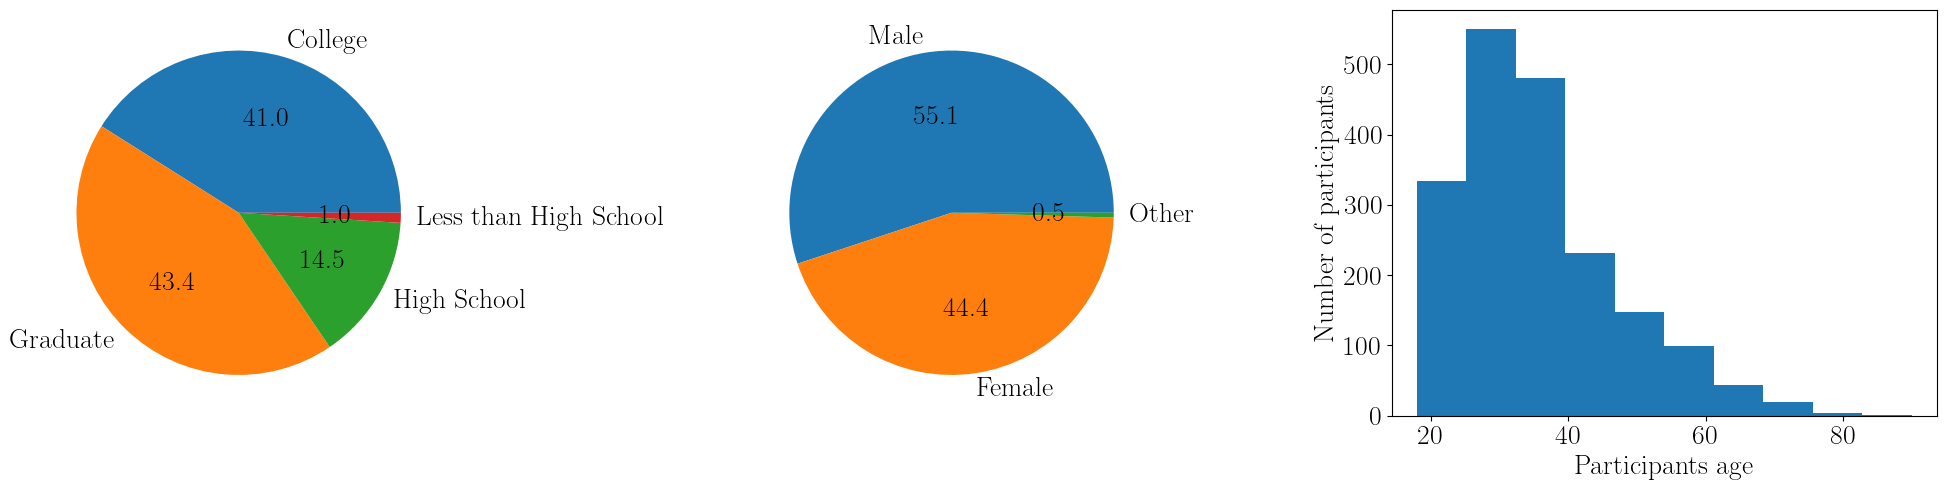
\includegraphics[width=15cm,height=4cm]{experiment/dists.png}
\caption{Distribution of education (left), gender (middle) and age (right) of participants. 
}\label{fig:distribution}
\end{center}
\end{figure}

The small elections (\textsc{Small-A} and  \textsc{Small-B}) consist of 10 candidate projects while the larger elections  (\textsc{Large-A},  \textsc{Large-B}) have 20 projects, all with a budget of $500,000$.
Project descriptions and costs were taken from real participatory budgeting elections from across the world.  
Each project was assigned a location on a map of the  city  and categorized in one of five  categories   (education; streets and transportation; culture and community; facilities and recreation; environment, public health and safety).  
Full  details  on every election including the project titles, descriptions,  costs and locations appear in the appendix.\rf{appendix}


 
Participants were first presented with a written and video description of the PB voting task and asked to pass  a simple quiz about the task before proceeding. 
Next, participants complete  the voting task  in their allocated PB configuration.
Each participant is assigned a  (random) location on the city map and   shown the description and location of the projects. 
We expect that a voter's location relative to  the project may affect their   preferences (e.g., people may prefer to vote for a library  close to their current location). 
  

 Figure~\ref{fig:interface} shows the interface  presented to participants who were asked to cast knapsack votes. 
 The left-most column shows the instructions and an indication of what fraction of the budget remains to be allocated. The center column shows the category and title of each proposed project, and a participant can click on a project to see a more detailed description. The right-most panel shows a map of the city on which the locations of the voter and the projects are marked (hovering over a project highlights its location). The other interfaces used in the study appear in the appendix. \gb{Note:appendix} 
 Project costs are  displayed for \points{} and \vfm{}, where it is needed to form a vote. 

  \begin{figure*}[h]
\begin{center}
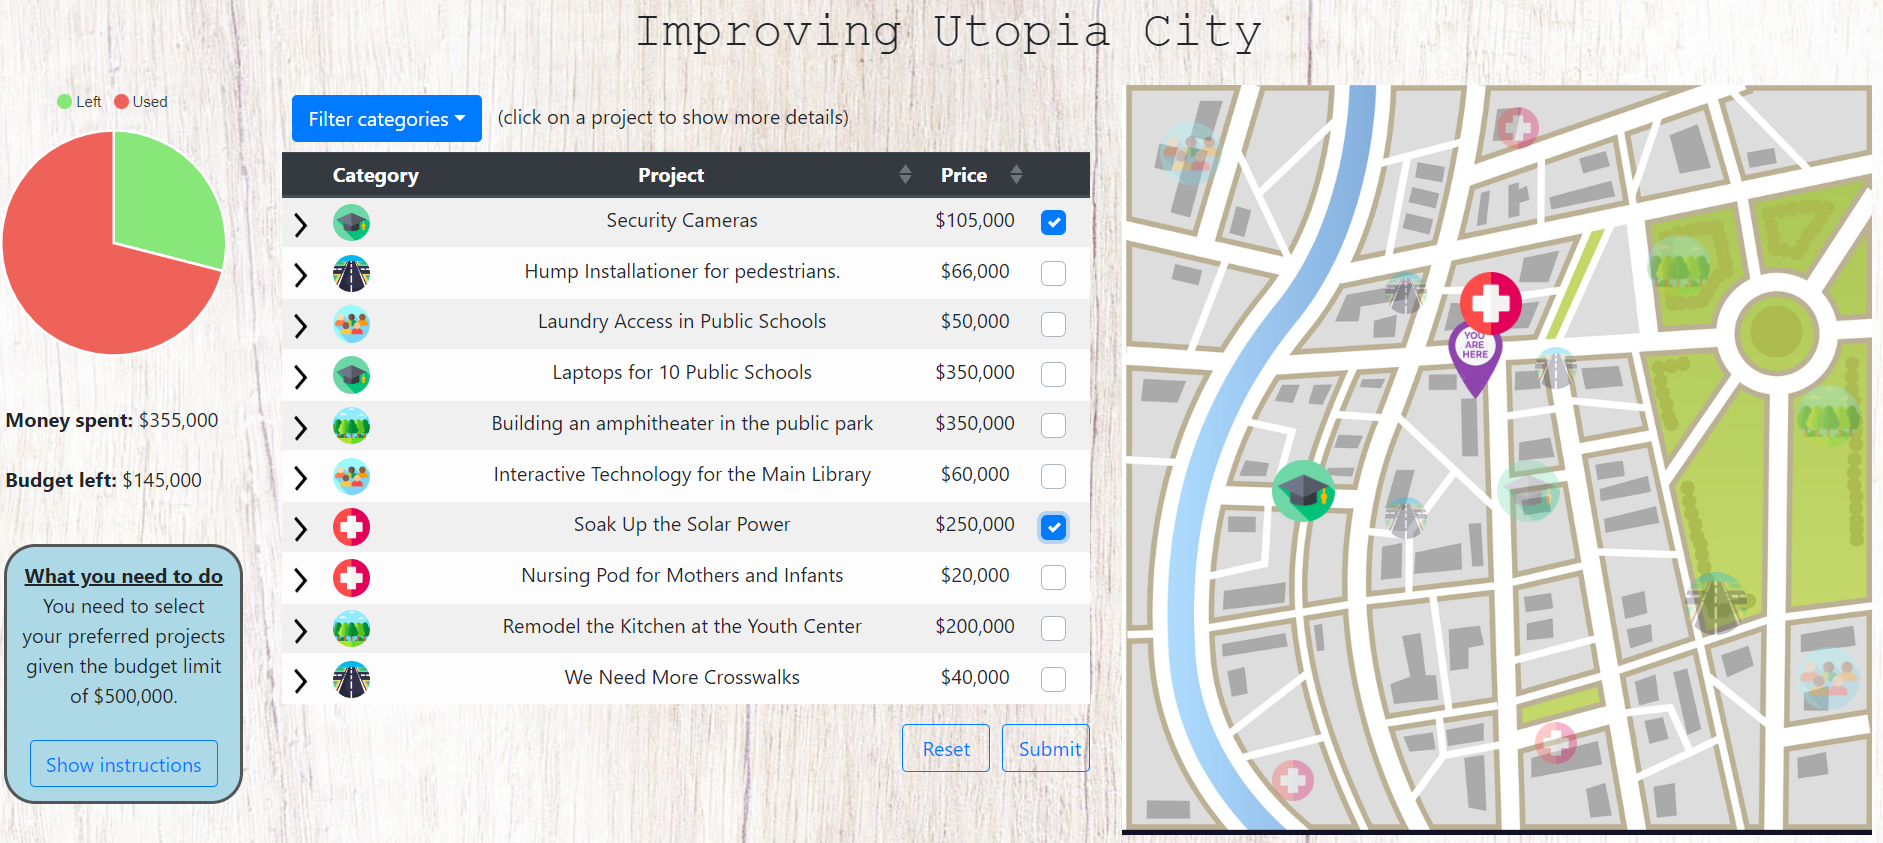
\includegraphics[clip, trim=0 3mm 0 0, width=15cm]{../experiment/full system.PNG}
\caption{The GUI for the \knap{}  input format (center), showing  the city map (right) and budget (left).
}\label{fig:interface}
\end{center}
\end{figure*}
 
 After   submitting their PB vote, participants  answer several consistency questions about their vote      designed to identify voters who vote randomly or carelessly (exact questions can be found in the appendix).\gb{note-appendix}
 Finally, participants   complete a short survey about their subjective experience of voting in the assigned format. They are asked to rate (on a scale of 1 to 5) how easy they found the task, how much they liked the user interface,   how   expressive  they found the input format,  and how much the project categories and their location on the map    affected their decisions (exact questions appear in the appendix). \gb{note-appendix} 
 
 Participants are rewarded a  fixed sum    for participation and  receive a 75\% bonus for passing the  consistency questions.  IRB approval was obtained from the corresponding institution. 

 
%%%%%%%%%%%%%%%%%%%%%%%%%%%%%%%%%%%%%%%%%%%%%%%%%%%%%%%

\subsection{Effect of Input Format on Voter Experience} 

 
We investigate the practical effects of using different input formats by comparing  the experiences of voters using the respective input formats.

This comparison has several components. Objectively, we record the time that it takes a voter to complete each of the first three stages of the task (completing the tutorial, answering the post-tutorial quiz, and casting a vote).  
We also report the number  of participants who fail the post-task consistency test and argue that a participant's inability  to recall simple information about the vote they just cast is correlated with the participant finding the task taxing, confusing or tiresome. 
More subjectively, we examine participants' self-reported scores from the post-completion survey.  

\subsubsection{Response Time}
The time it takes to complete a task is a recognized  proxy for  the cognitive burden  or difficulty of the task  \citep{rauterberg1992method}.  
%
The average time to complete each stage of the experiment is visually represented in  Figure~\ref{fig:time}.  Results in this section are averaged across elections and the conclusions do not change when looking at any individual election. %\gb{May be worth just looking at times for large vs small to see if there is anything interesting}

Participants voting in  the \vfm{}   format are consistently slowest to complete each stage of the experiment, suggesting that voters find \vfm{}  very hard to use. Based on the time it takes to cast a vote,  \points{} and \tapp{} are the next hardest formats to use. In the former case, this provides some evidence for the widely accepted belief  that asking voters for cardinal utilities is infeasible; in the latter, it  highlights the complications that sprout from  \tapp{} requiring cross-voter normalization and the fact that  \tapp{} is a relatively niche format which voters are unlikely to have encountered before.  
Voters found \kapp{} the easiest to use, followed by \knap{} and \rank{}.

\begin{figure}[t]
\begin{center}
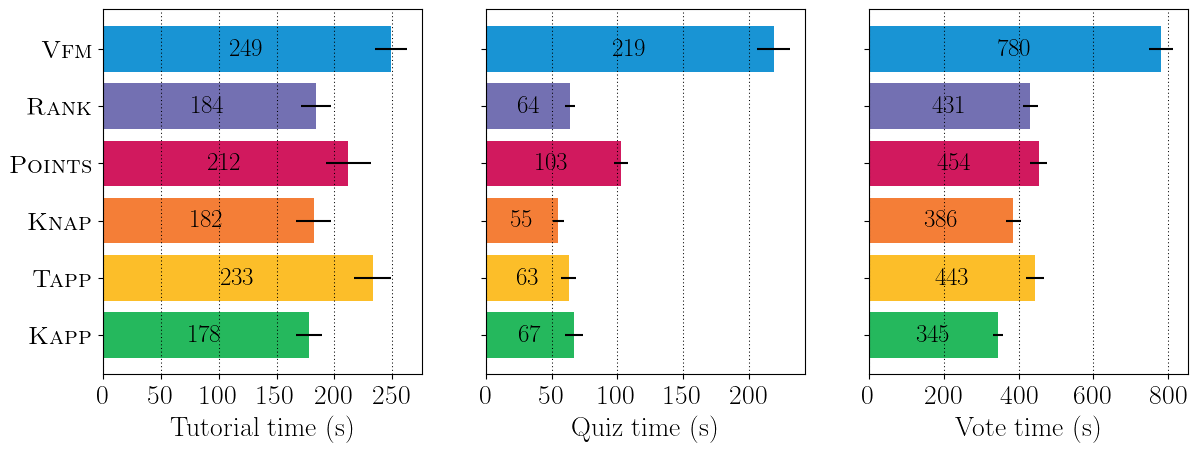
\includegraphics[width=15cm,height=5cm]{../experiment/time_combined.png}
% 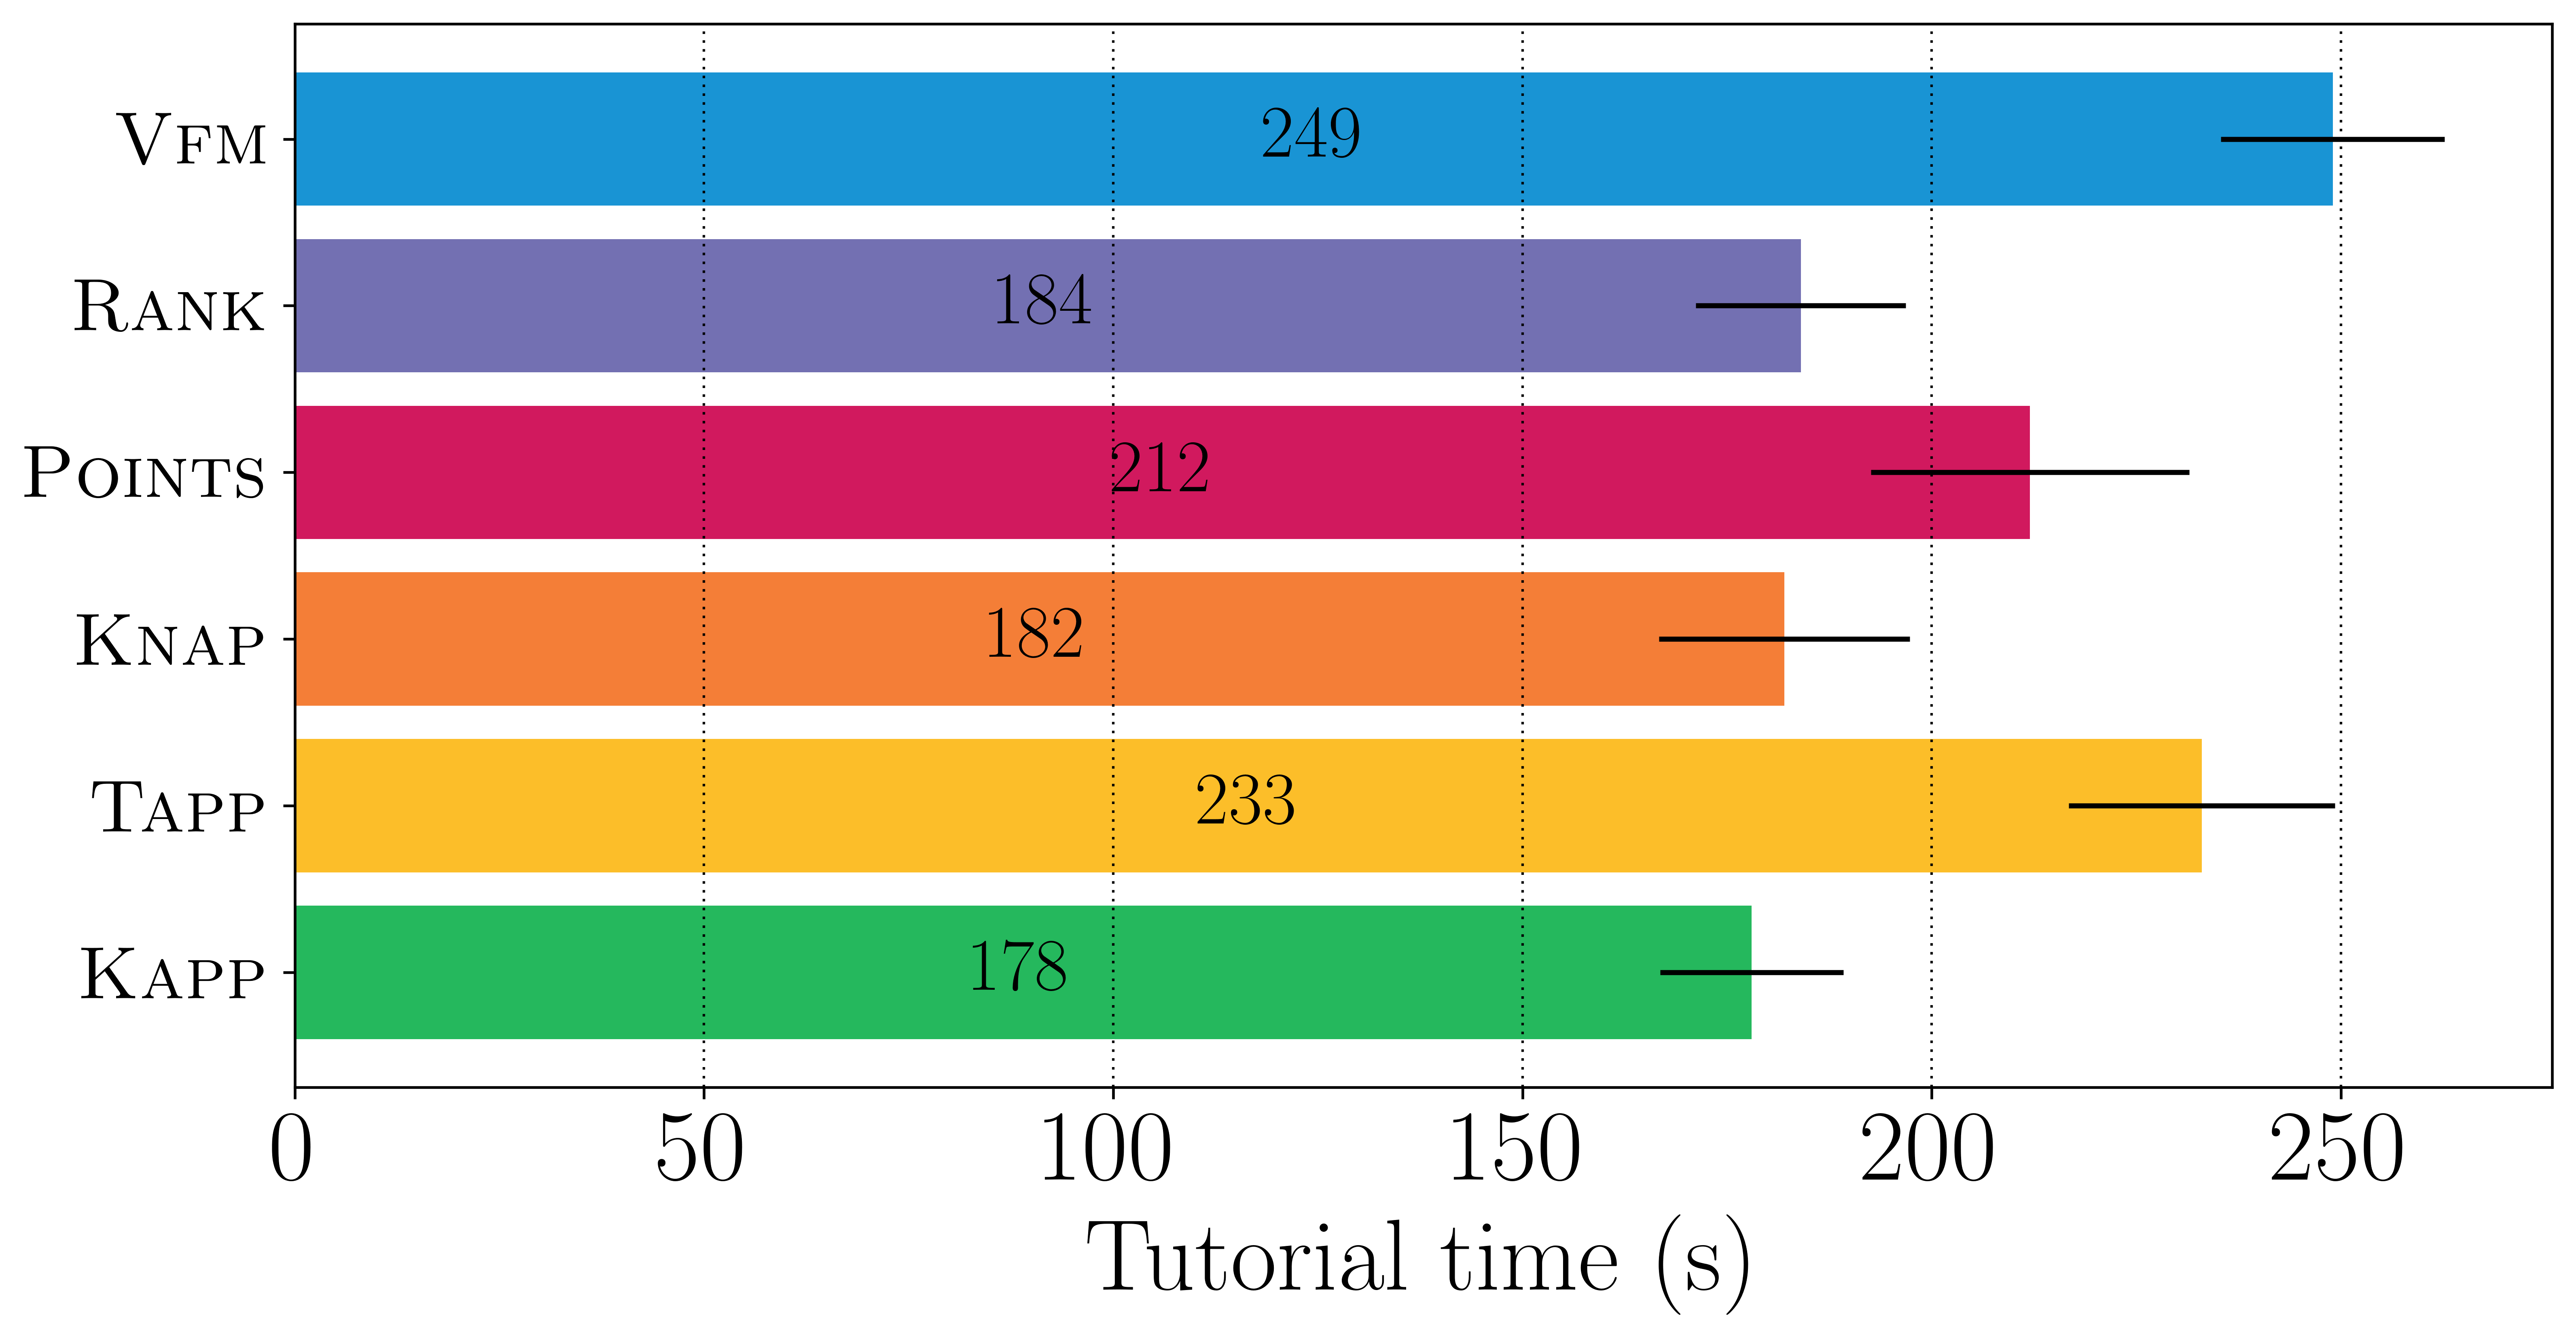
\includegraphics[width=5cm,height=4cm]{../experiment/tutorial_time.png}
% 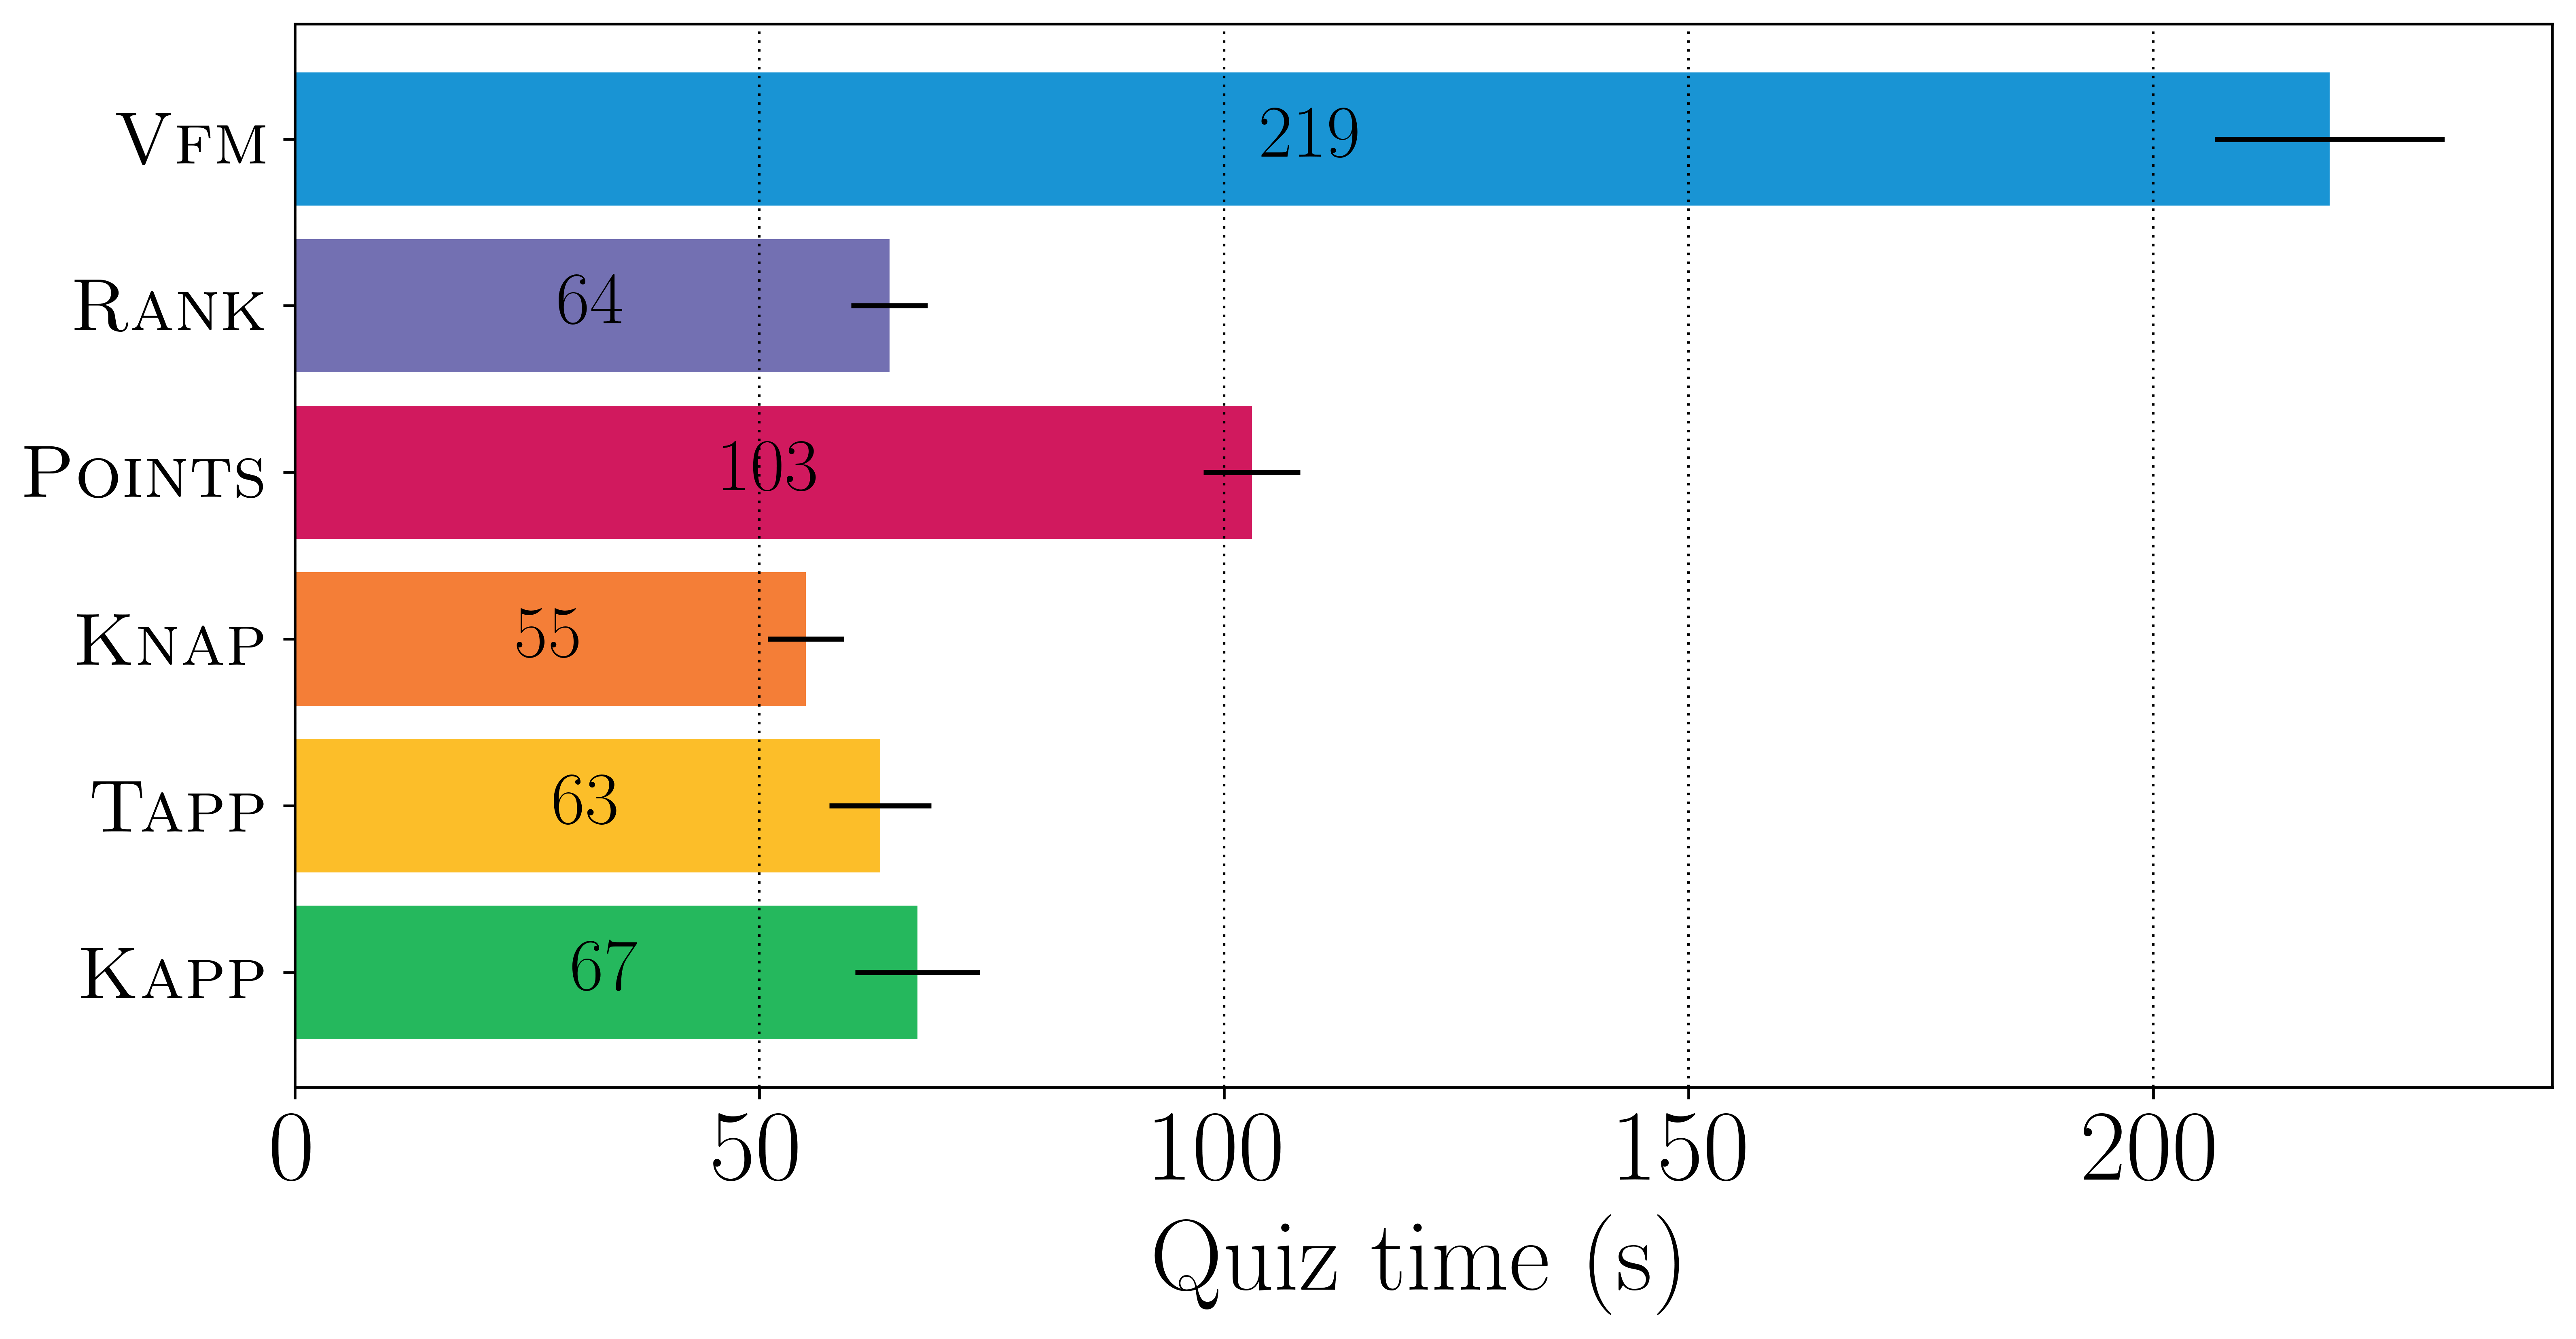
\includegraphics[width=5cm,height=4cm]{../experiment/quiz_time.png}
% 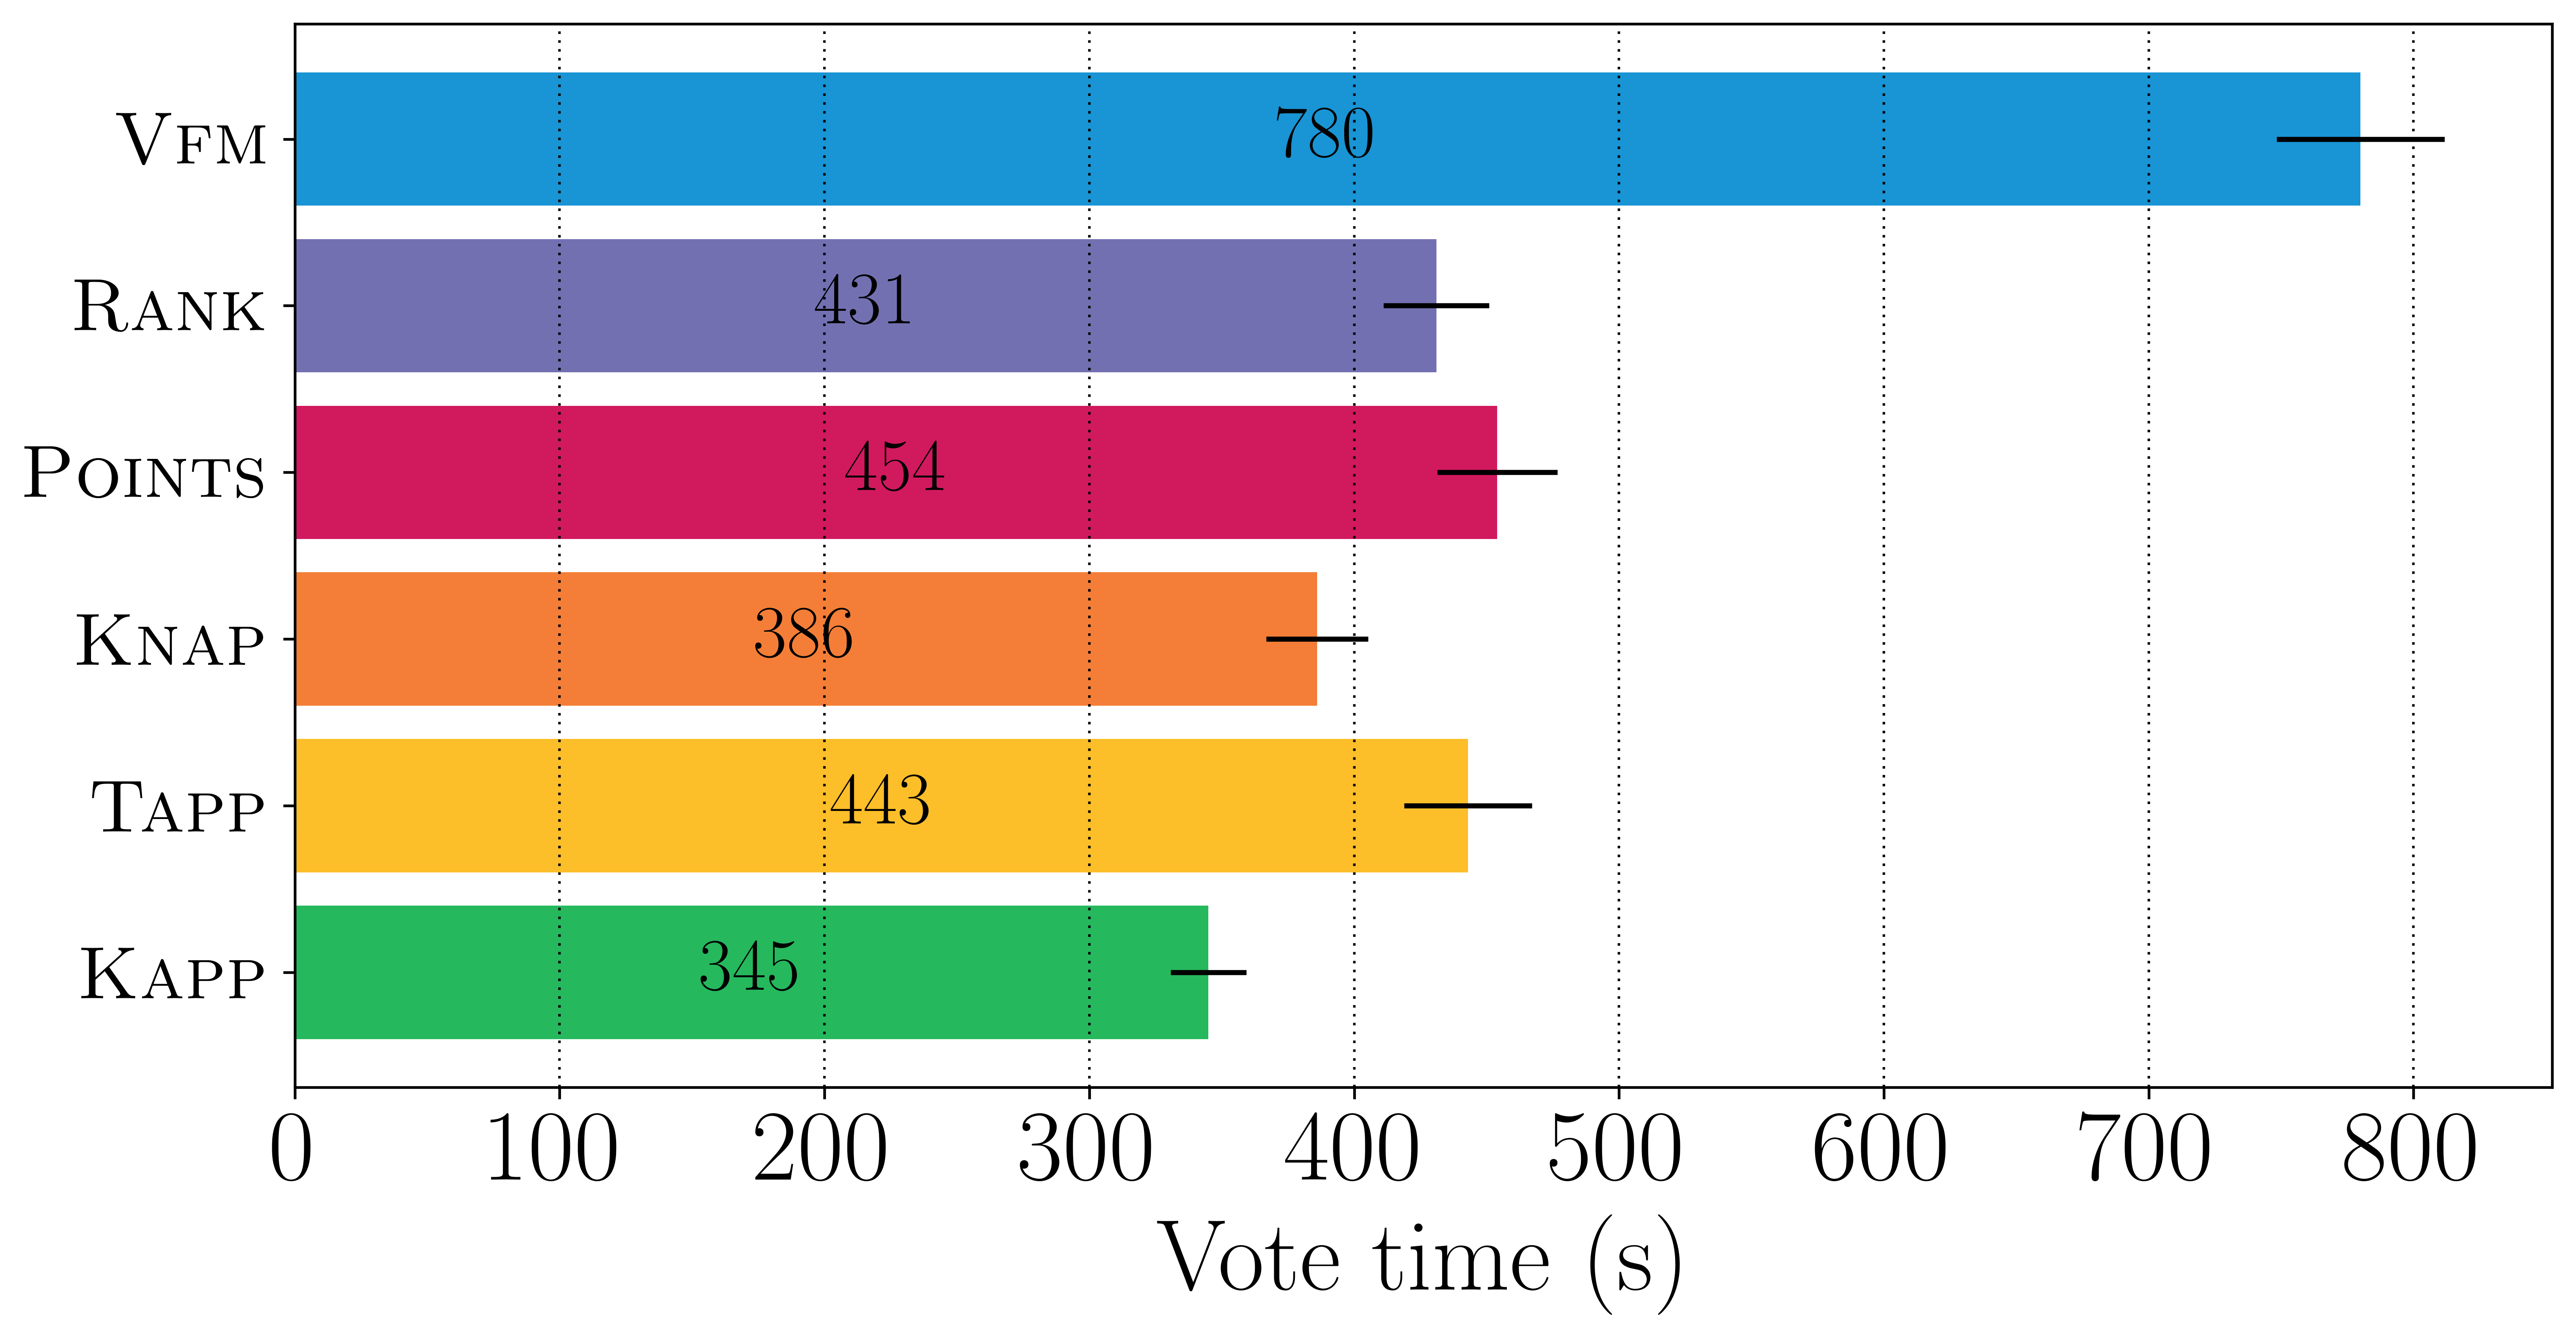
\includegraphics[width=5cm,height=4cm]{../experiment/vote_time.png}
\caption{Average time ($s$) to complete each stage of the task. 
}\label{fig:time}
\end{center}
\end{figure}

\subsubsection{Consistency Checks}
 
Of the roughly 75 participants  recruited for each of the 24 configurations of the experiment, on average 58 passed the consistency test. 
%
The consistency test  is designed to check whether the participant can recall simple information about the recently completed task. 
%
There are several reasons why a voter may fail the test. For example, they may answer randomly in order to complete task quickly,  become  distracted  if the task is too tiresome, or confused if the input format is hard to understand. As such, we  treat this as another signal about the difficulty of expressing  preferences in a given format. 

%We  compare the rate of passing the consistency test across input formats. 
Participants using the ranking-based formats are most consistent, followed by the approval-based formats.  We speculate that the high consistency of \vfm{} is, at least in part, thanks to the inordinately long amount of time voters spend considering their votes. Users of \points{} are comfortably the least consistent, which  supports earlier evidence that providing cardinal utilities is a challenging task.
%
There is very little variation in the rate of passing the consistency test across the four elections. A complete breakdown of the results appear in the appendix. \gb{note-appendix} 

 

\subsubsection{Self-Reported Voting Experience}
In addition to the time it took participants to complete the task and how much they could recall about their submitted preferences, we also expressly asked them to rate various aspects of the experience on a scale of 1 to 5. 
Survey results are summarised in  Figures~\ref{fig:feedback} and \ref{fig:cat_map}. 
Results for the questions omitted from this discussion appear in the appendix. \gb{note-appendix}
We test for statistical significance with a Kruskal–Wallis test to show the input formats give different results, followed by a Dunn test for post hoc comparison.
All of the survey questions   gave $p < 0.004$  for the Kruskal test. The Dunn test evaluated statistically significance   at the $p < 0.05$ level.



\textbf{Ease of use}  We ask participants  how easy they found the voting task. Unsurprisingly, participants found \vfm{} significantly harder to use than any other format. \points{} was rated as quite easy to use despite being one of the more time-intensive formats. \kapp{} was rated as significantly easier to use than all other  formats except \points. 



\textbf{Perceived expressiveness} We ask  participants how well they felt their vote captured their preferences. 
Participants found \kapp{} to be most expressive and, in particular,  significantly more expressive than  \tapp, \vfm, and \points. It is somewhat surprising that \kapp{} was rated as more expressive than \points, since you can infer a \kapp-vote from  your \points-vote; we speculate that the relative complexity of  \points{} explains part of this phenomenon. It is also possible that participants conflated expressiveness and ease of use, or failed to consider alternatives to the format presented to them.
\vfm{} is perceived to be least expressive by some margin. Again, the  difficulty of using \vfm{} and the fact that voters are forced to explicitly consider project costs may have contributed to the perception that it is less expressive than \rank, which also asks for a ranking of alternatives.  


\begin{figure}[htb]
\begin{center}
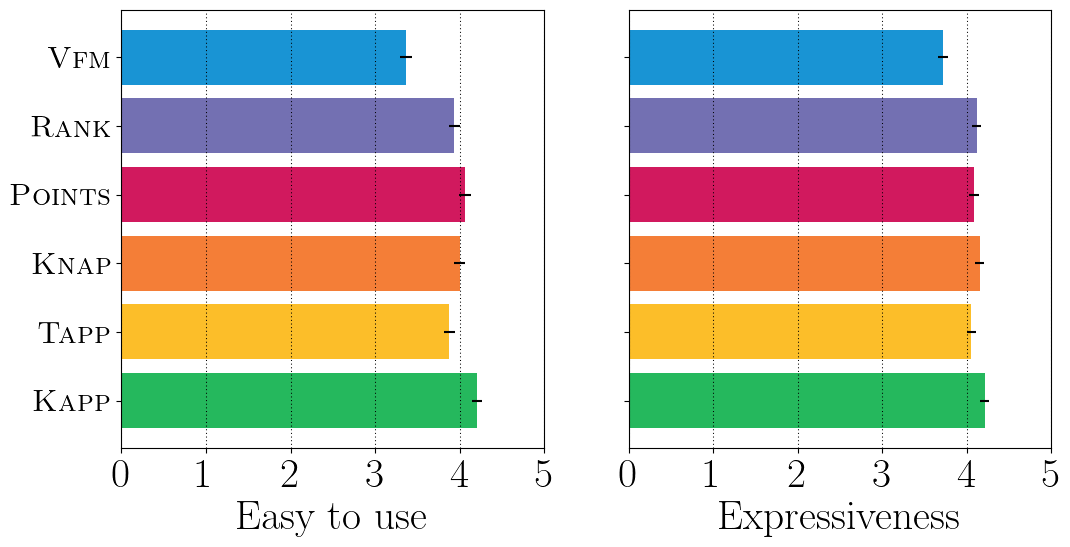
\includegraphics[width=8.5cm]{../experiment/survey1.png}
\caption{The average feedback for each input format.
}\label{fig:feedback}
\end{center}\vspace{-3mm}
\end{figure}

\begin{figure}[htb]
\begin{center}
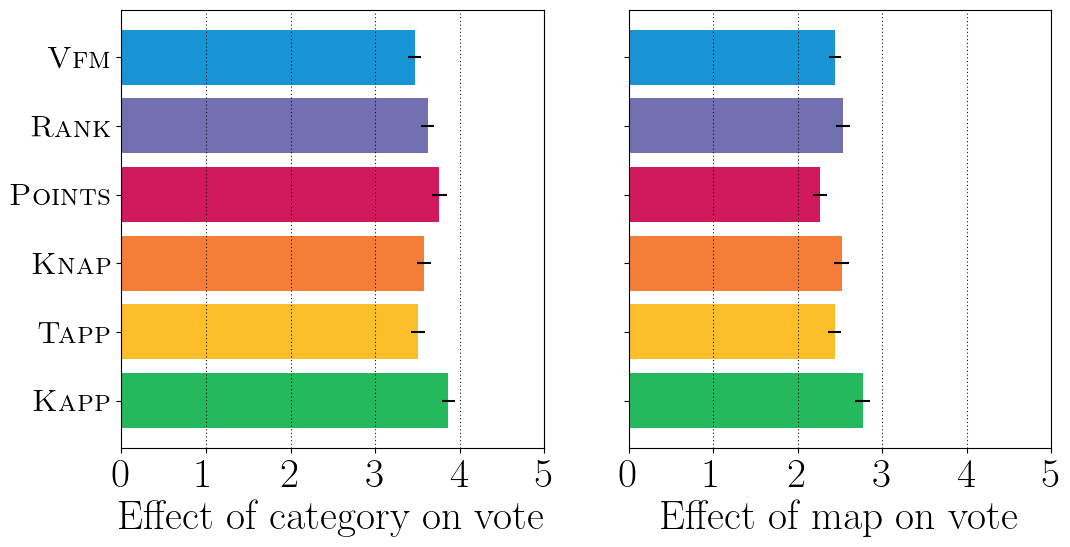
\includegraphics[width=8.5cm]{../experiment/survey2.png}
\caption{The average effect of the categories and the map.
}\label{fig:cat_map}
\end{center}\vspace{-5mm}
\end{figure}


\textbf{Effect of additional information}
Projects were assigned to one of five categories (e.g.\ transport or education) and given locations on a city map. Two survey questions asked about the extent that project categories and the map influenced participants' preferences. These results are summarised in Figure~\ref{fig:cat_map}.
%
Participants using \kapp{} were influenced  more by project locations than any other group. Similarly, \kapp-voters paid significantly more attention to project categories than all other groups except \points-voters. 
We posit  that the \kapp{} format was easy enough to understand and use that it freed participants up to consider additional, non-core information about the projects and   election in their decisions. 


\subsection{Evaluating aggregation methods}
\label{sec:aggregation}

In this section we   start by comparing binary and cost-utilities, followed by a more fine-grained comparison of the greedy and and ES aggregation methods. 

\subsubsection{Welfare and representation}
An obstacle to comparing outcomes based on social welfare is that participants are assigned only one format, so there is no common basis of comparison when aggregating vote profiles from different formats. To address this, we make the assumption that, since voters are randomly assigned to input formats, the distribution of voter preferences are the same across formats. As such, we can deduce voter valuation functions from the full vote profile in \emph{any} format and treat these aggregated values as a proxy for the welfare of all voters, regardless which format they used.  We caution that this is, at best, a very coarse evaluation, since assuming a value based on  a vote in any of the formats requires very strong assumptions.  

We report in Figure~\ref{fig:exp:welfare} the   social welfare (averaged over the four elections) as measured when treating the full profile of \points{} (left) or \knap{} (right) voters as representative.  

\begin{figure}[htb]
\begin{center}
% 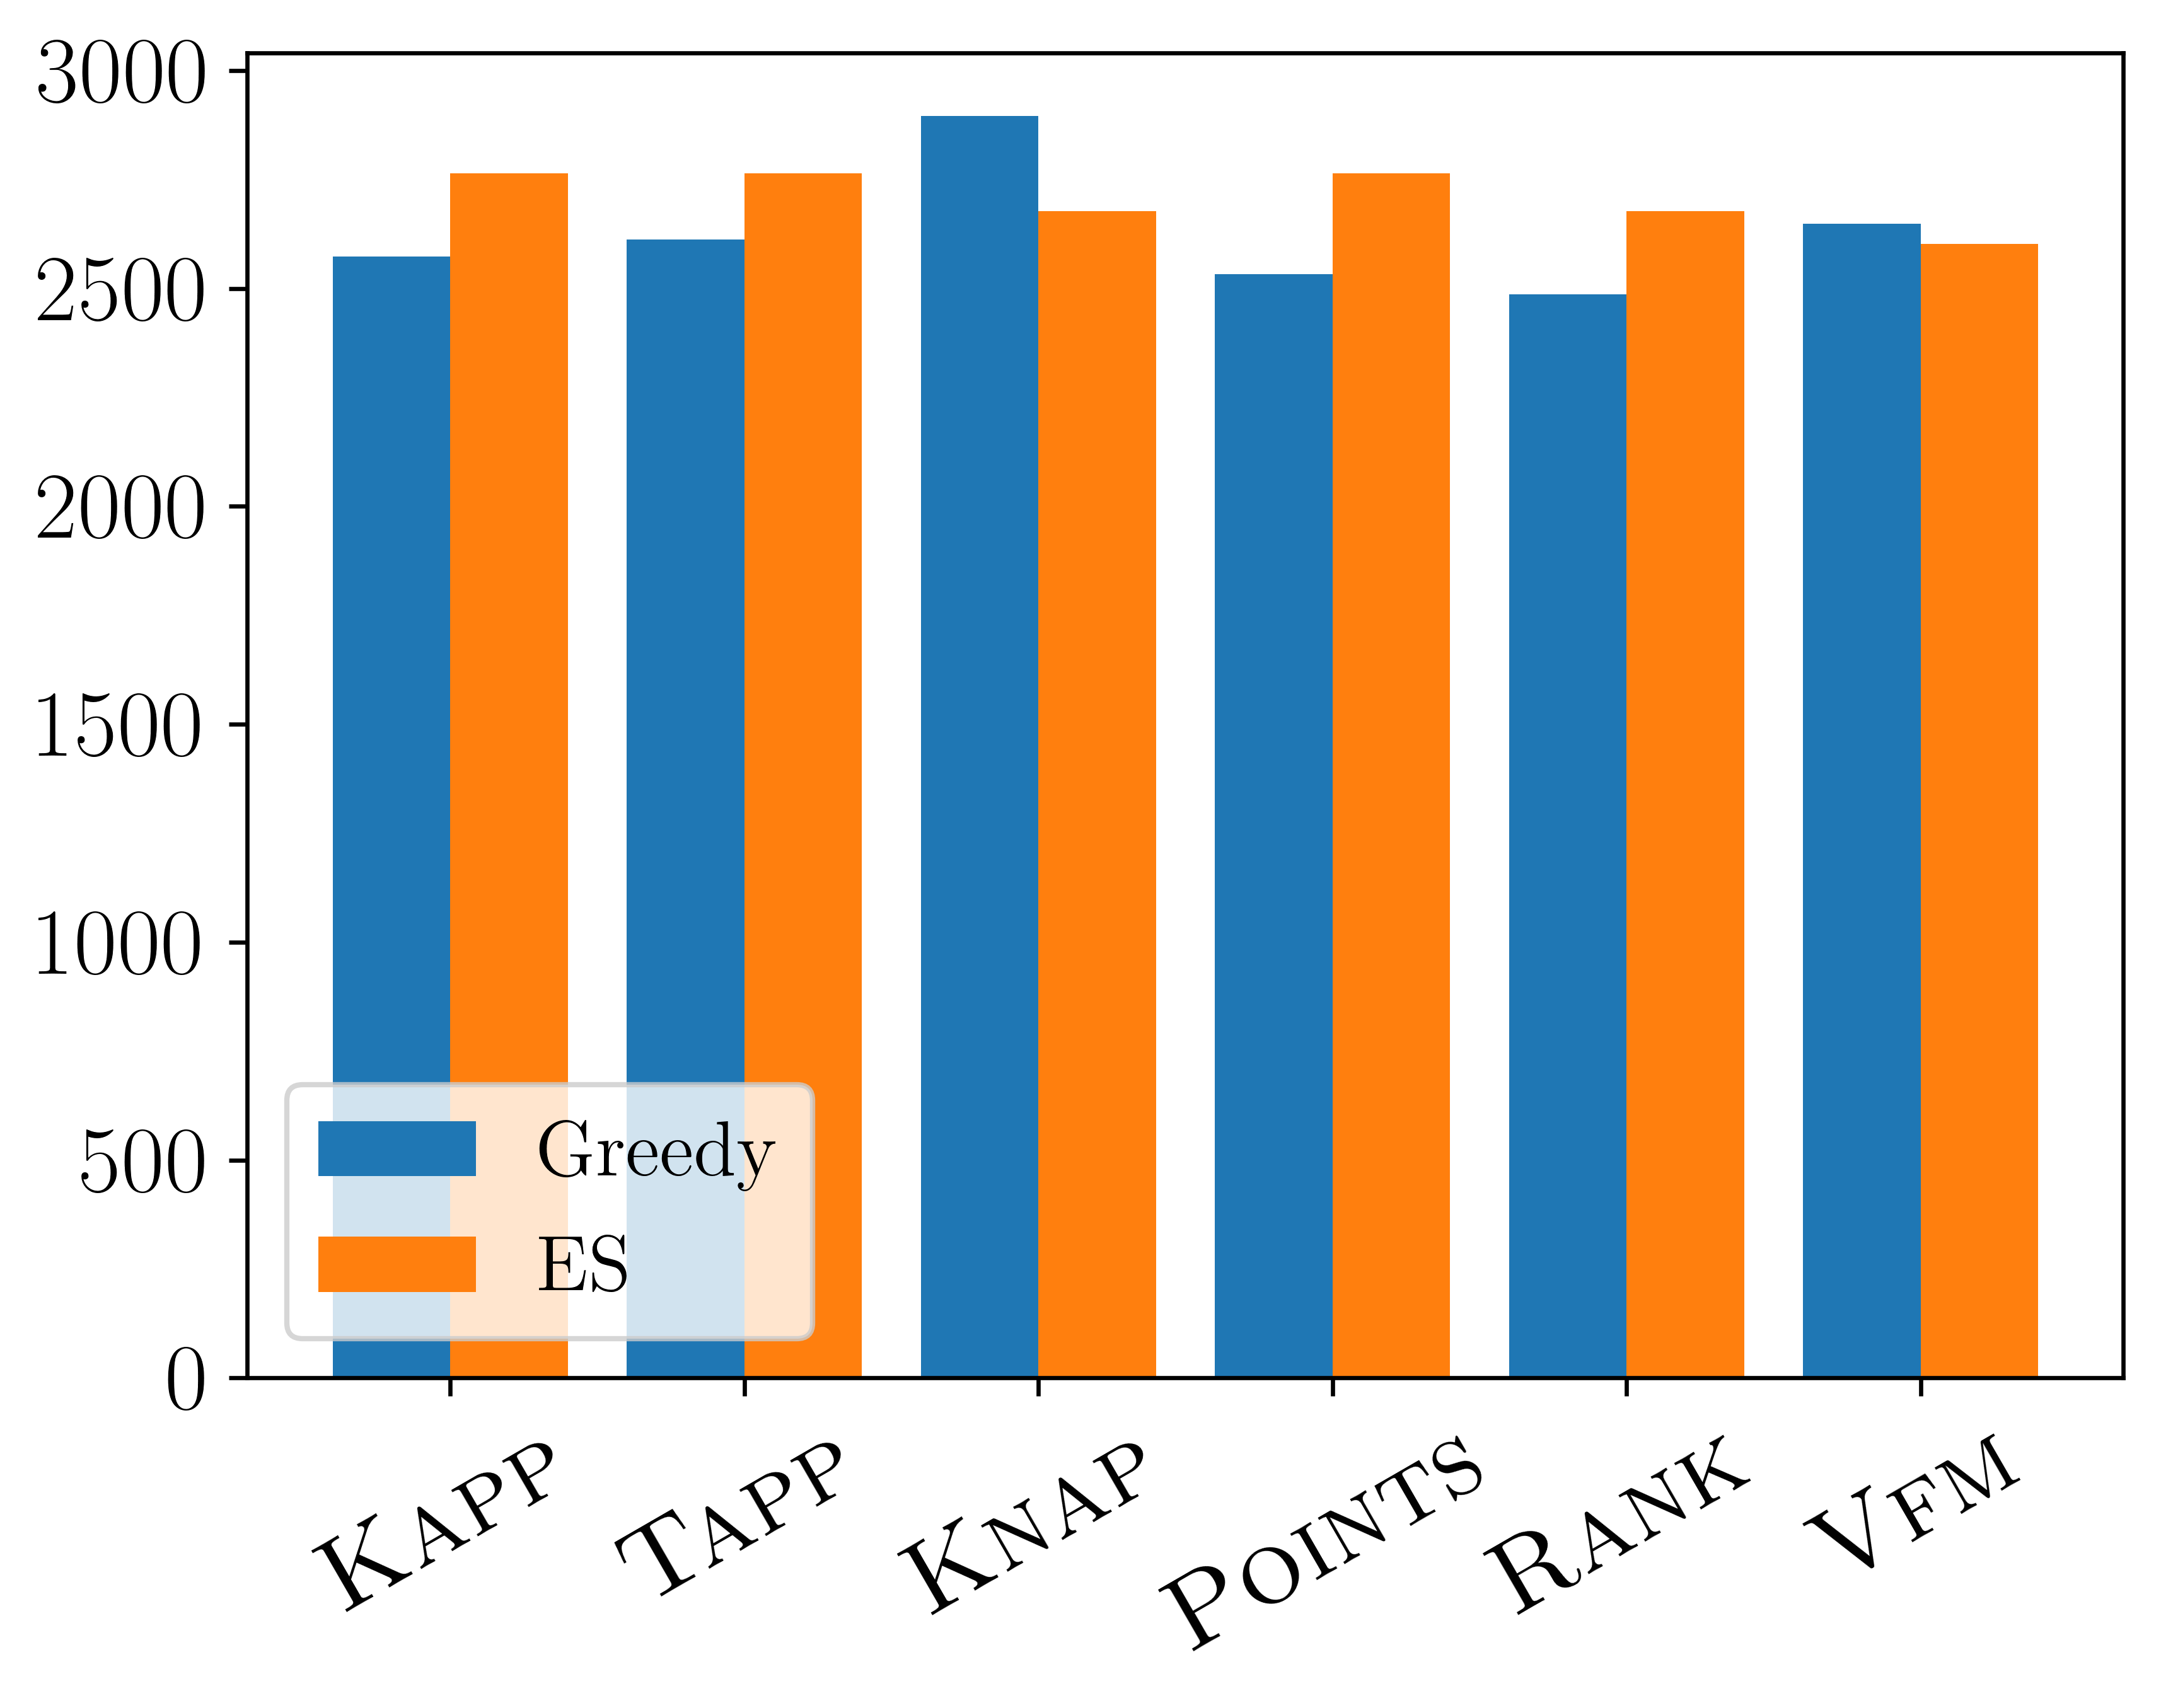
\includegraphics[trim={.8cm .5cm 1cm 1.3cm}, clip,width=4cm]{experiment/Utilities_welfare.png}
% 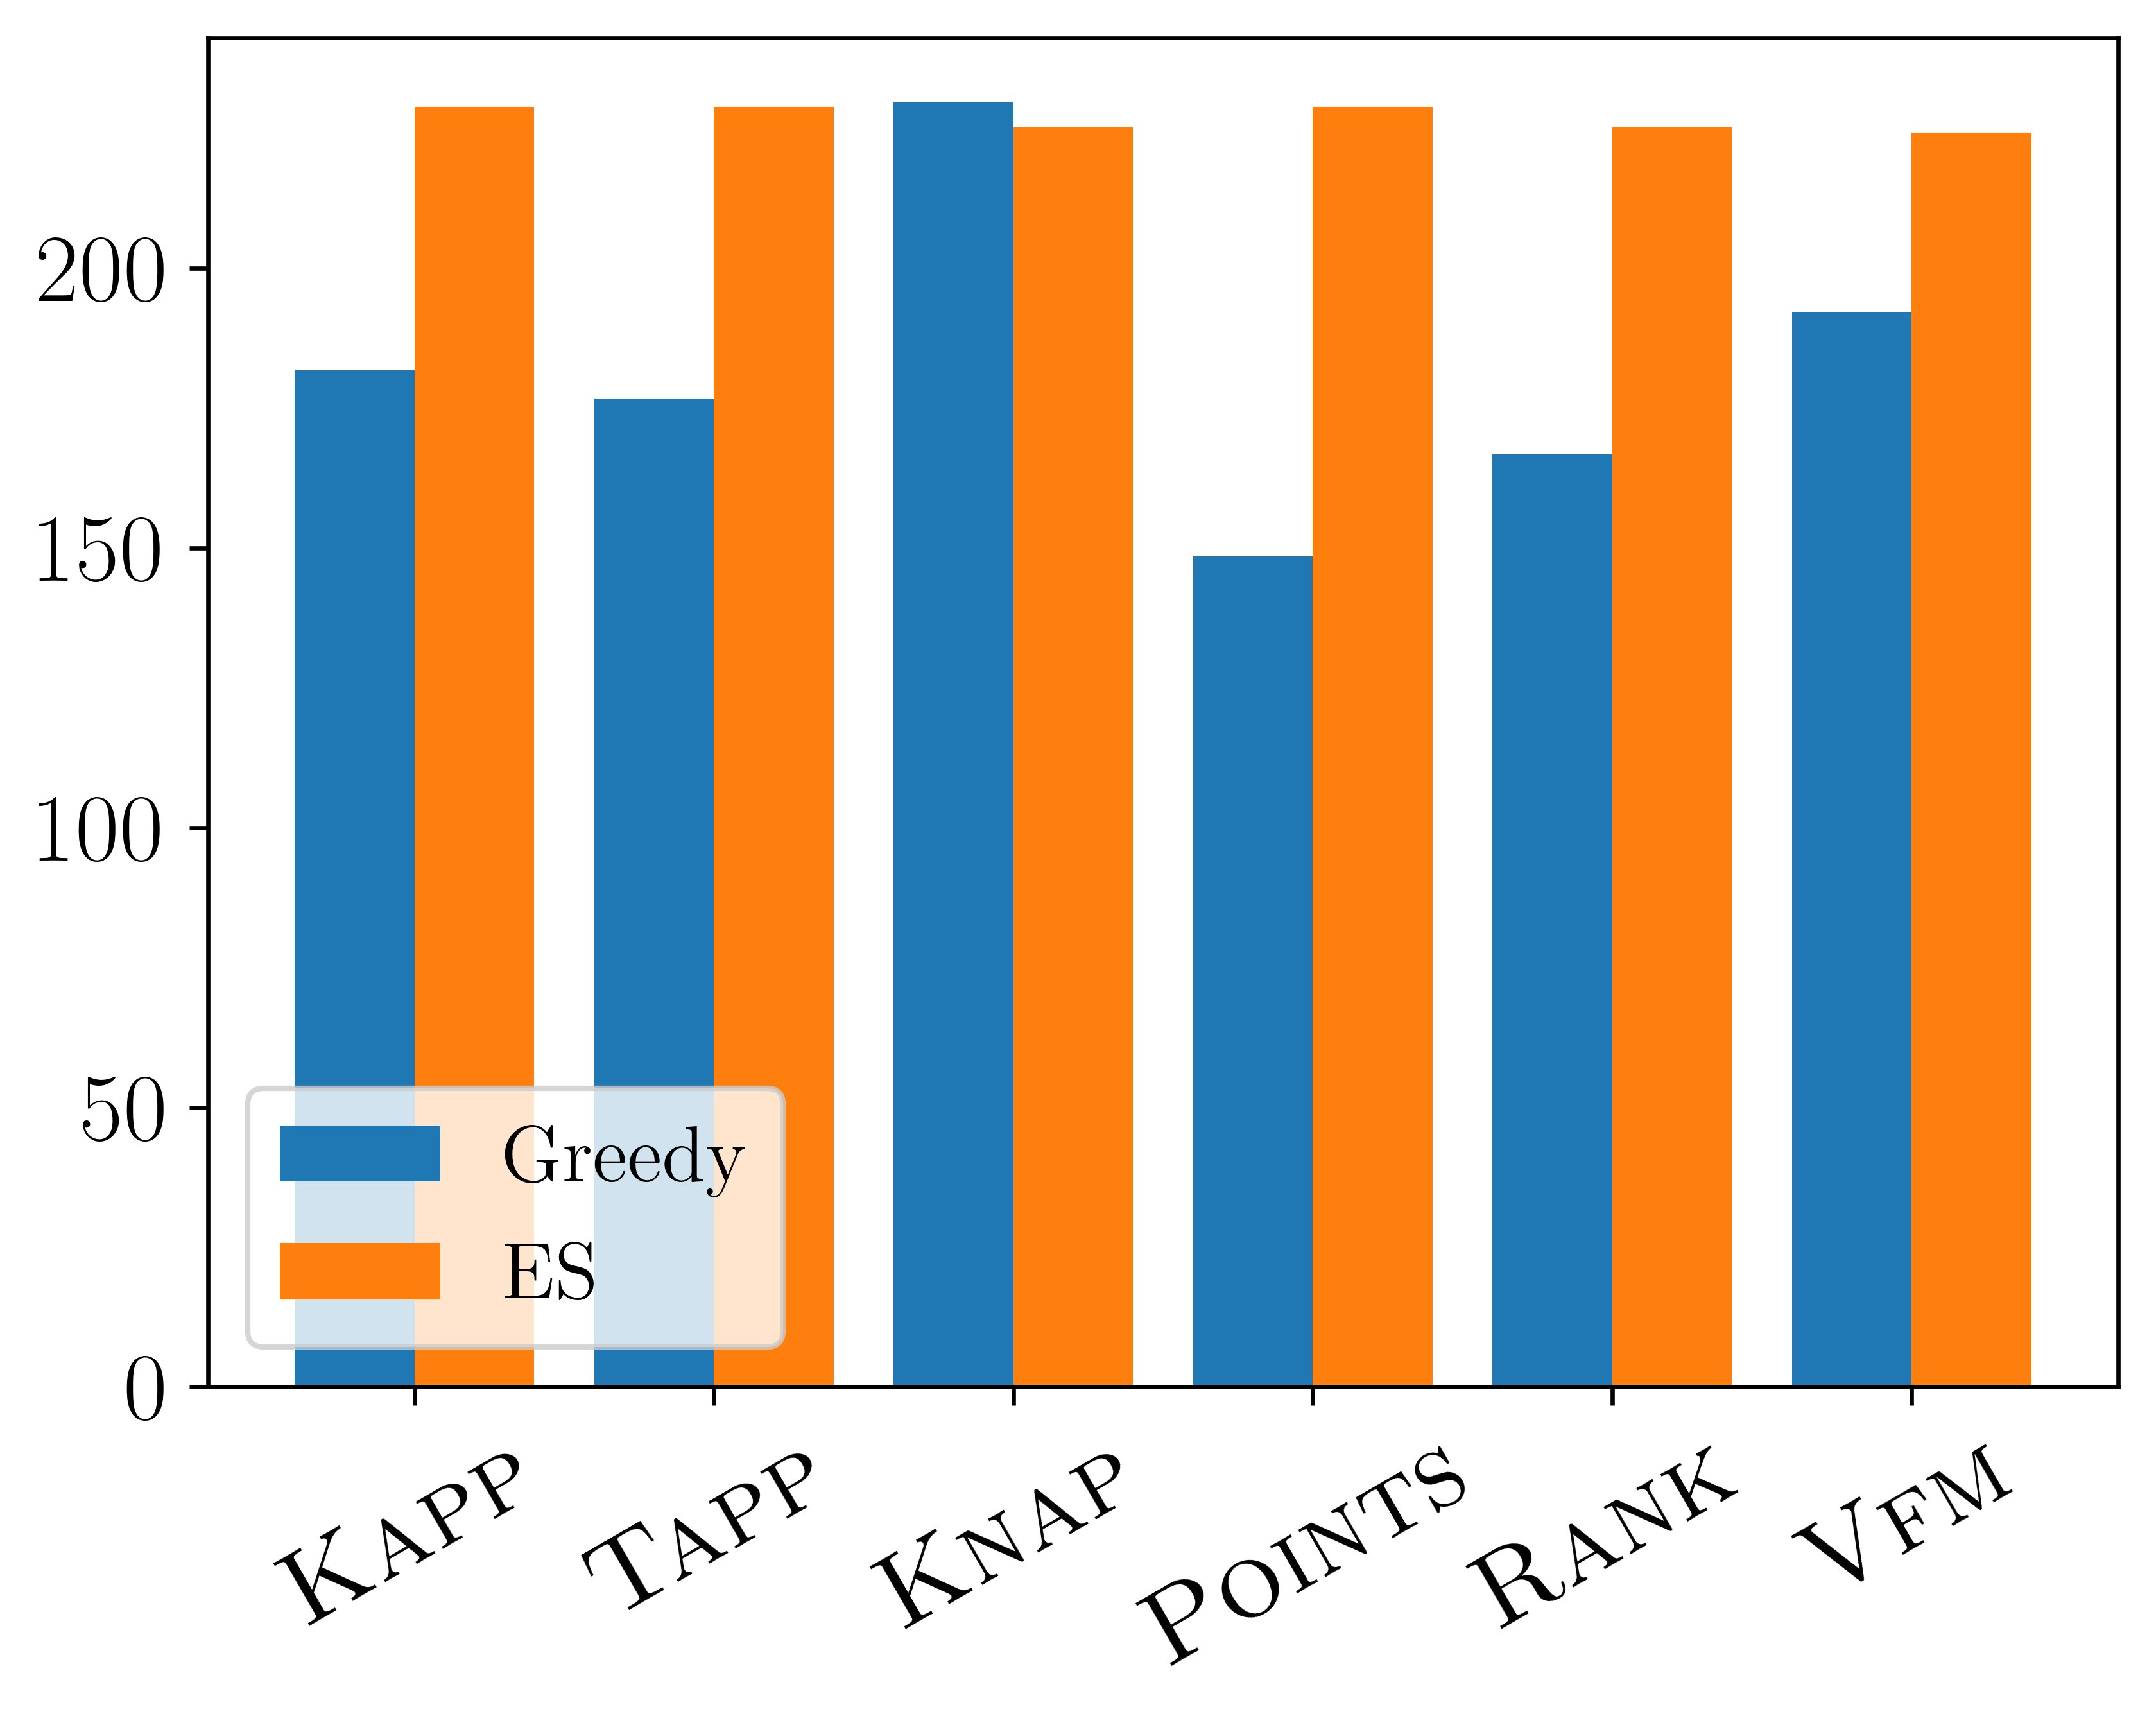
\includegraphics[trim={.8cm .5cm 1cm 1.3cm}, clip,width=4cm]{experiment/Knapsack_welfare.png}
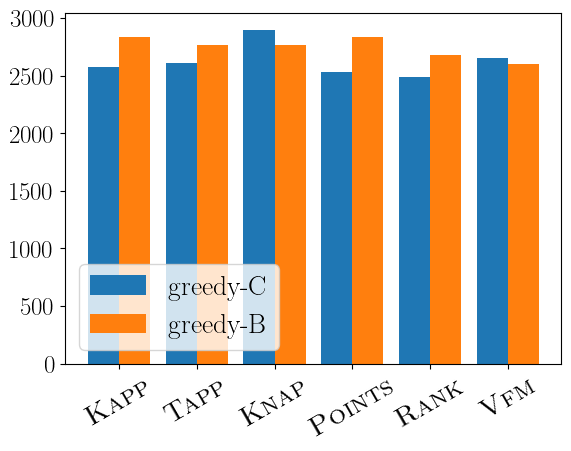
\includegraphics[width=4cm]{experiment/Utilities_greedy.png}
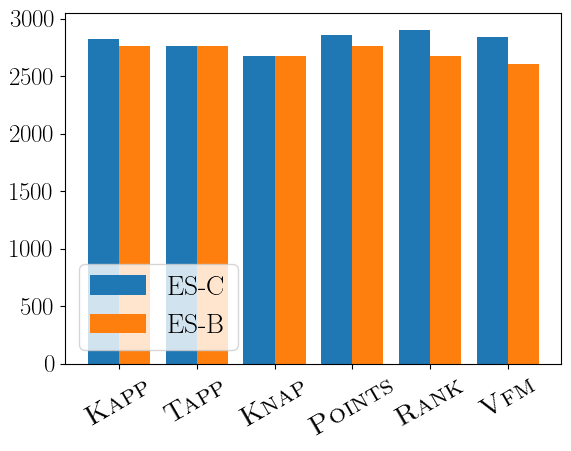
\includegraphics[width=4cm]{experiment/Utilities_ES.png}
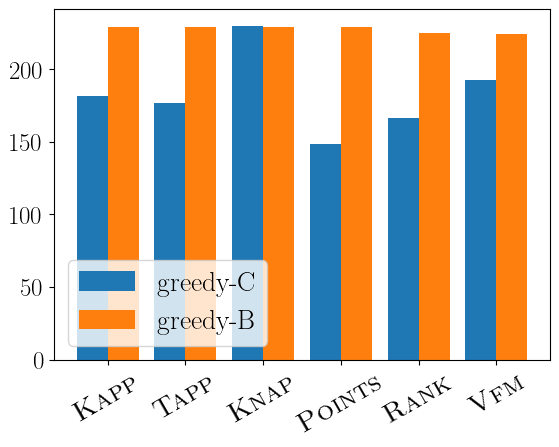
\includegraphics[width=4cm]{experiment/Knapsack_greedy.png}
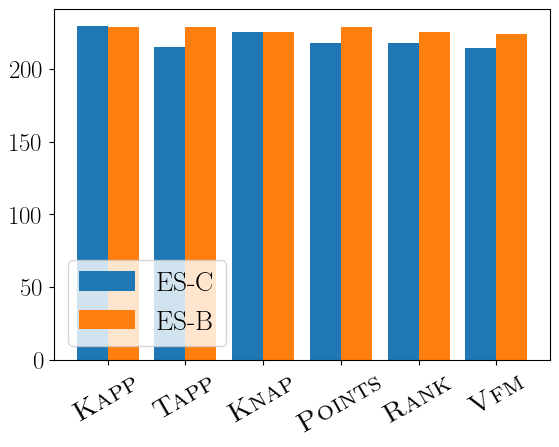
\includegraphics[width=4cm]{experiment/Knapsack_ES.png}

\caption{Average social welfare     using   \points- (left) and \knap-voters (right) to compute welfare. 
%todo 2 sets of 6 plots with, 1 set for 01 utilities, one for 0,cost. pick a couple for here, rest in the appendix. 
}\label{fig:exp:welfare}
\end{center}\vspace{-5mm}
\end{figure}

We find very little to distinguish between alternative configurations on the basis of welfare. Neither     aggregation method or utility function  strictly outperforms the other. Occasionally, when using greedy aggregation, the choice of input format can have a large effect on welfare. This is highlighted in Figure~\ref{fig:exp:welfare} when using \knap-voters to compute welfare. \bingreedy{} and both versions of ES  are less sensitive to  the choice of input format and   achieves very similar welfare across input formats.
Results when using the other formats to measure welfare are less extreme and appear in the appendix.\gb{appendix}

\begin{figure}[!t]
\begin{center}
% 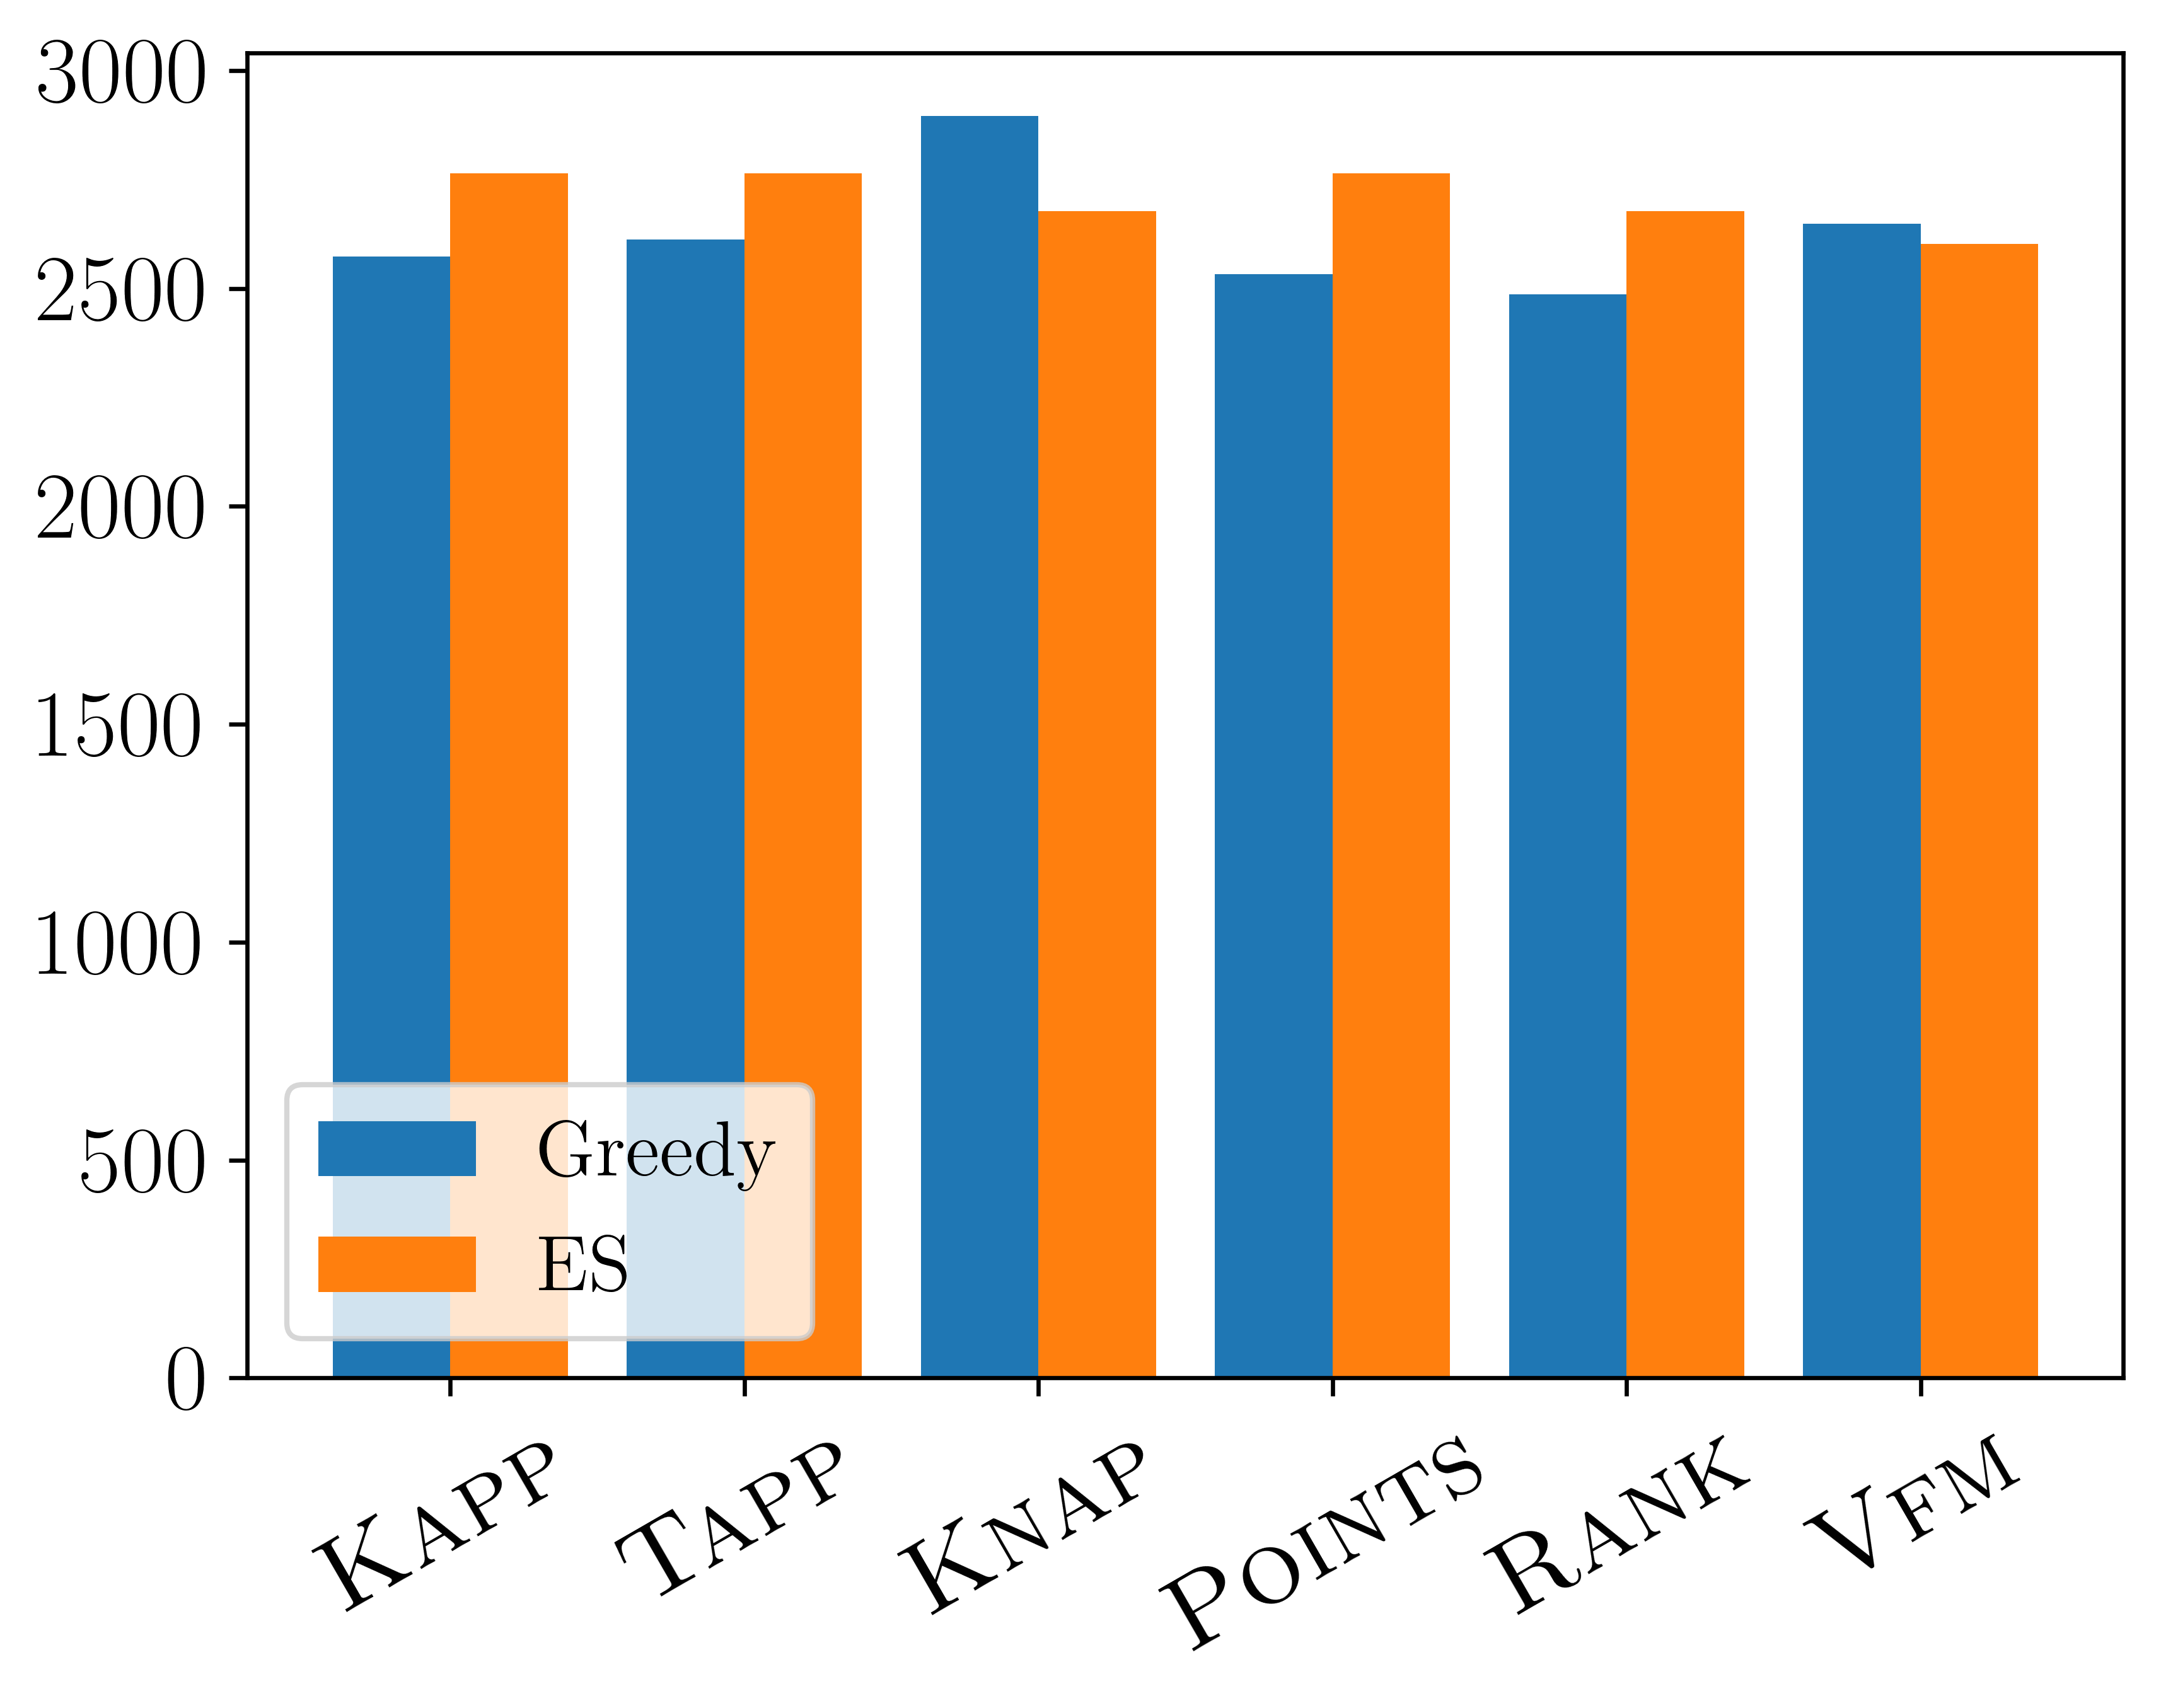
\includegraphics[trim={.8cm .5cm 1cm 1.3cm}, clip,width=4cm]{experiment/Utilities_welfare.png}
% 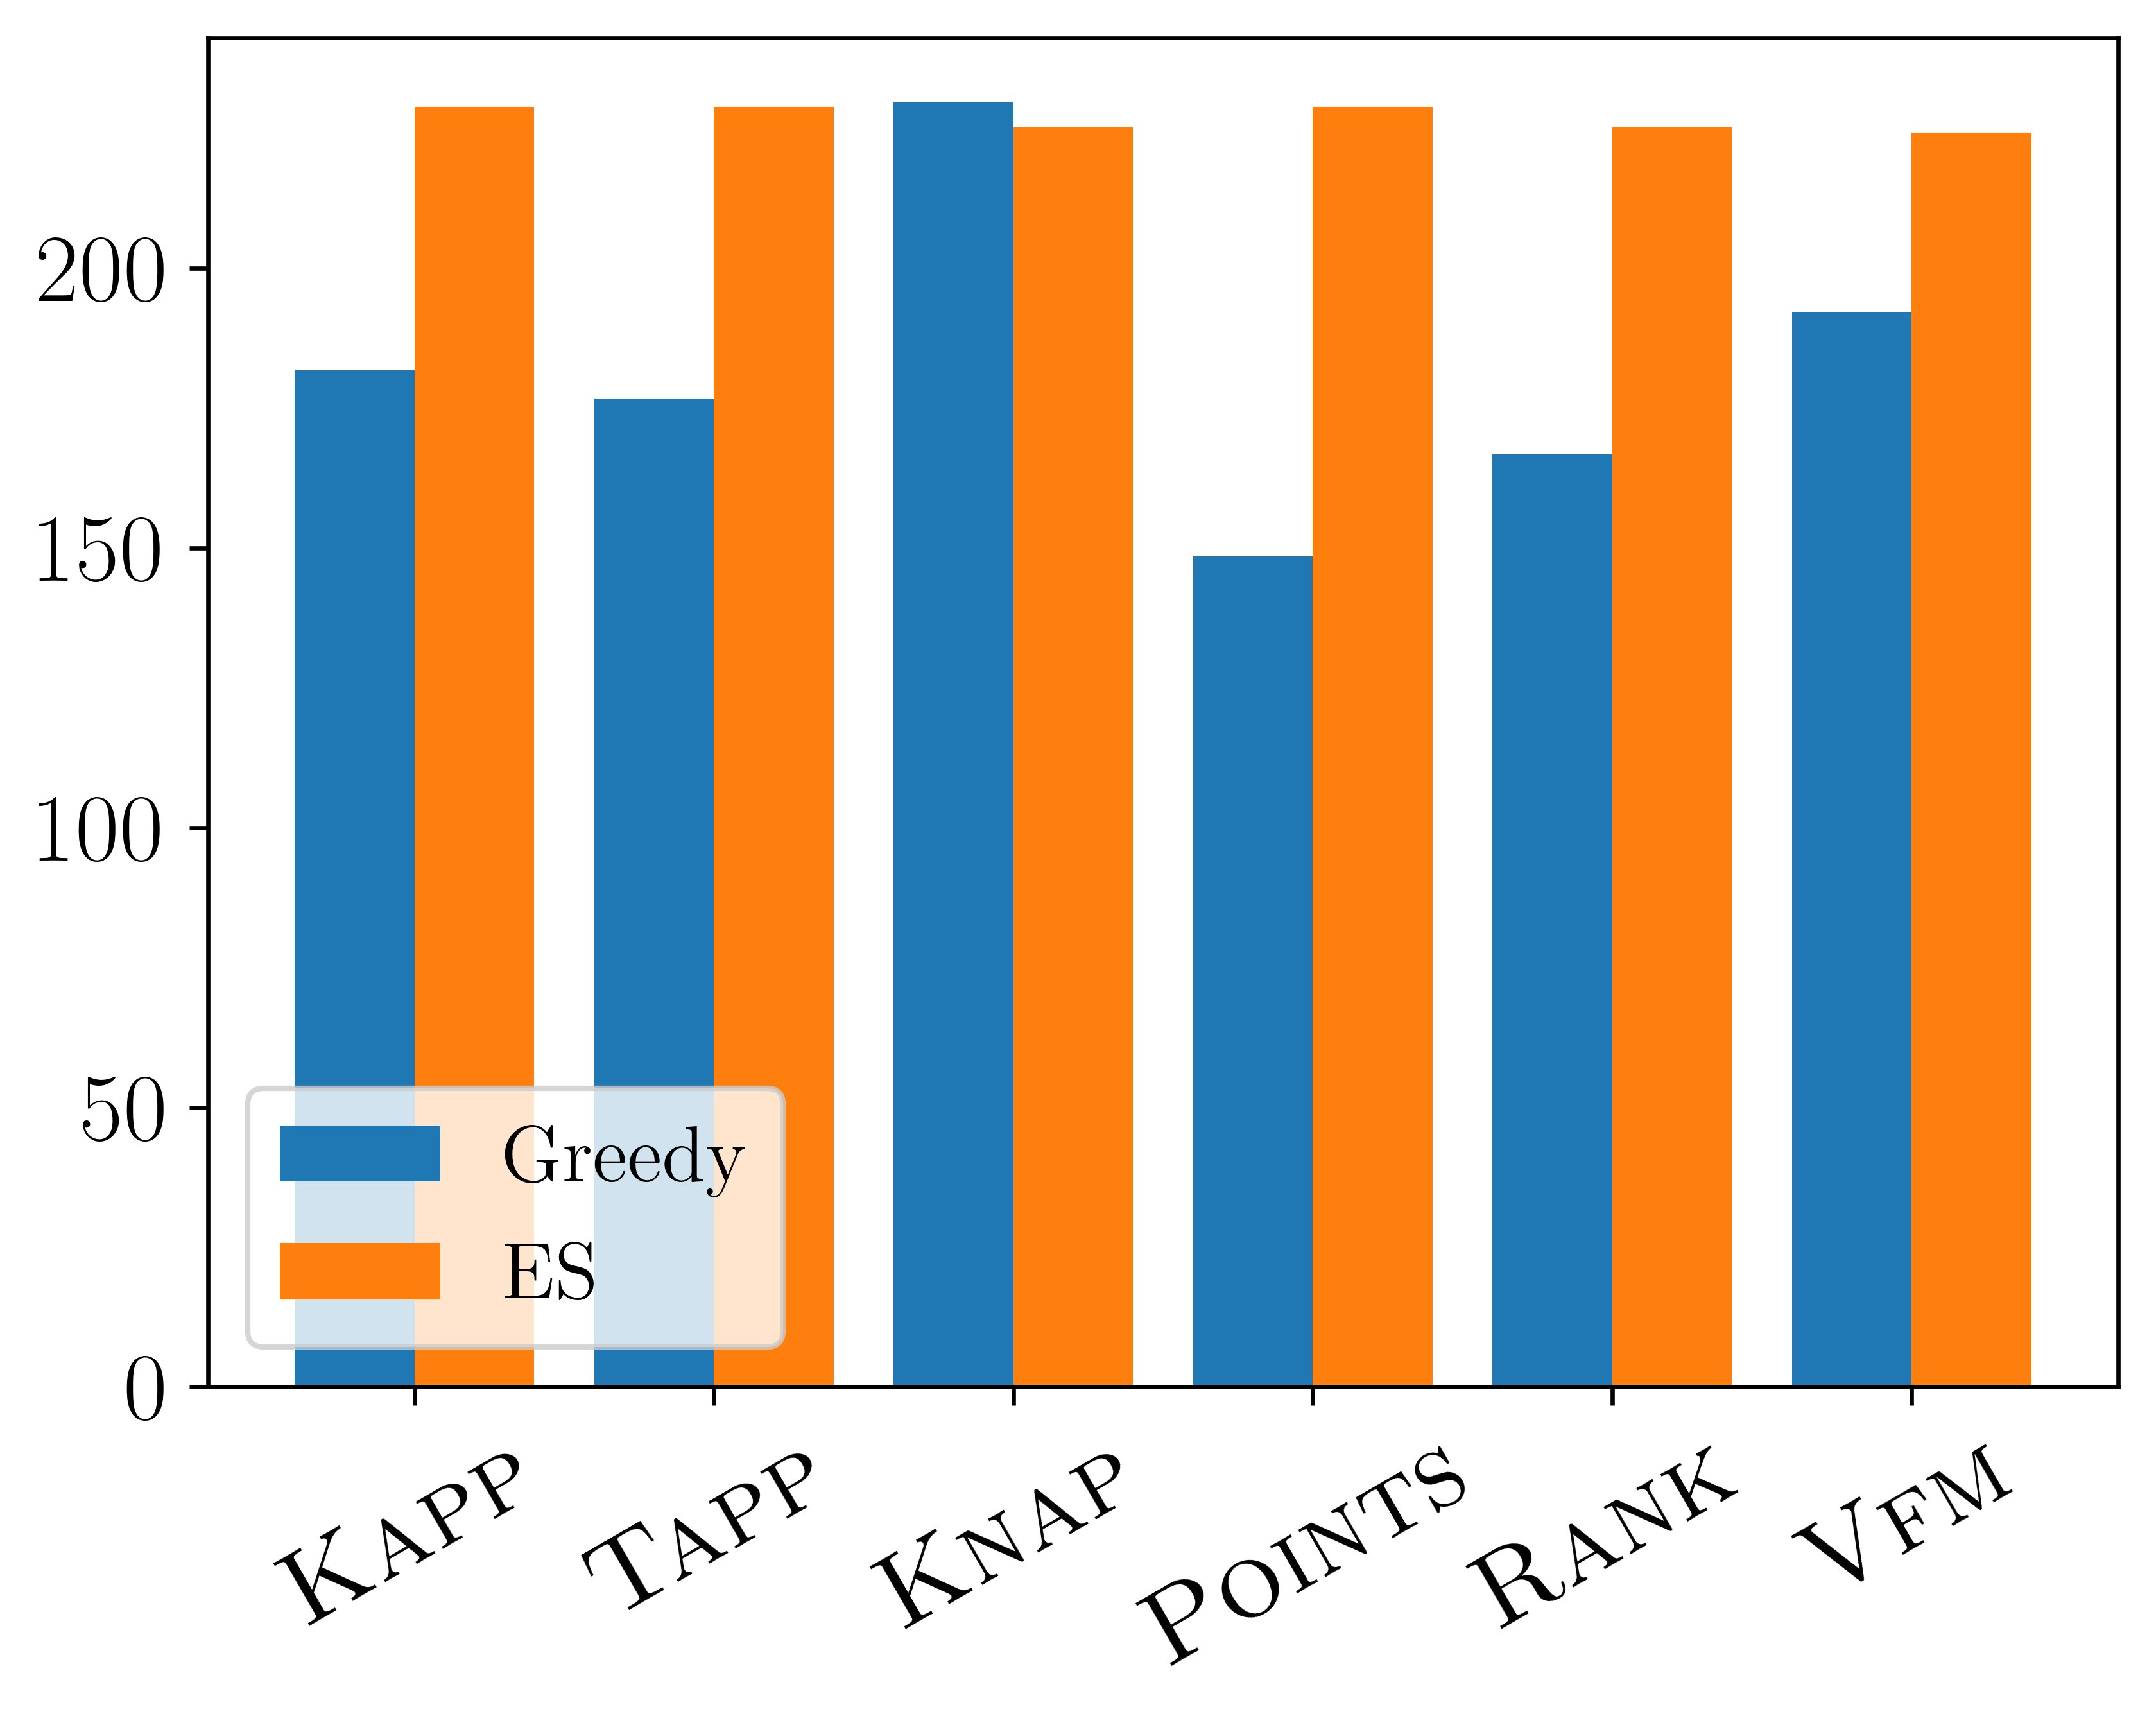
\includegraphics[trim={.8cm .5cm 1cm 1.3cm}, clip,width=4cm]{experiment/Knapsack_welfare.png}
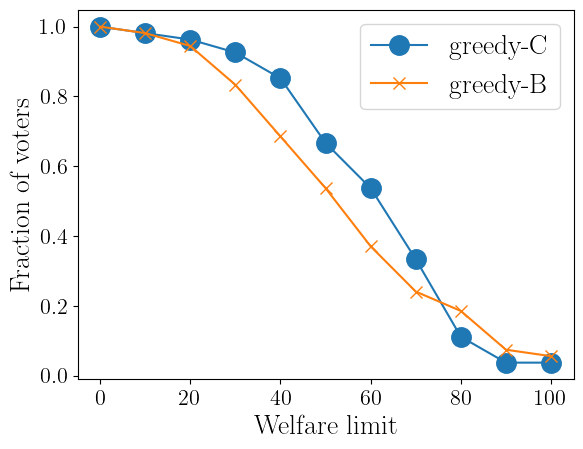
\includegraphics[width=4cm]{experiment/('Utilities', 6, 'Utilities')_greedy.png}
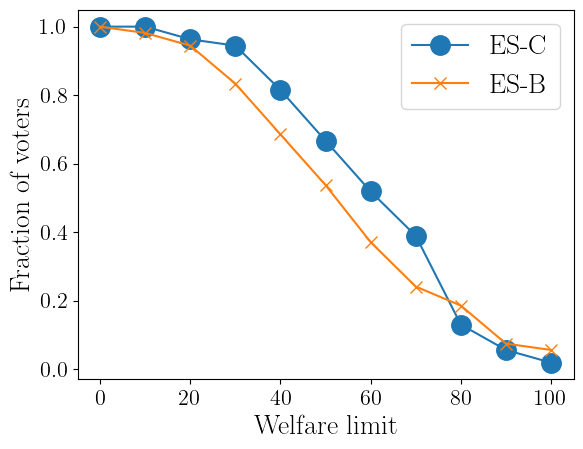
\includegraphics[width=4cm]{experiment/('Utilities', 6, 'Utilities')_ES.png}
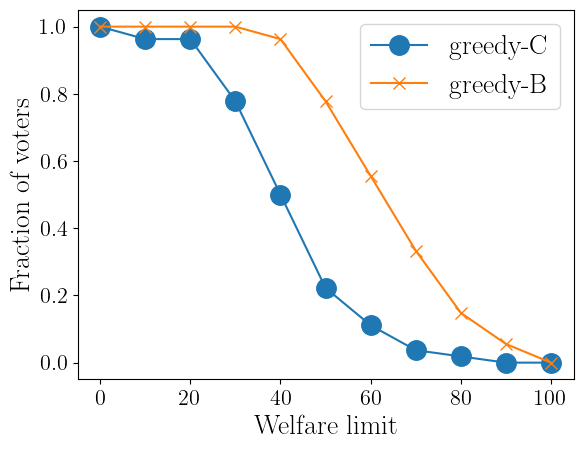
\includegraphics[width=4cm]{experiment/('Utilities', 7, 'Utilities')_greedy.png}
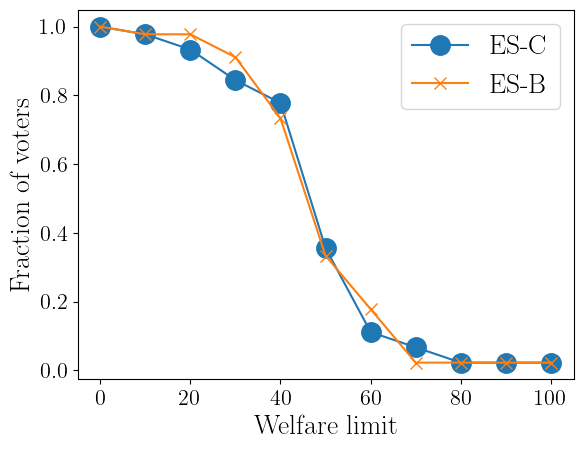
\includegraphics[width=4cm]{experiment/('Utilities', 8, 'Utilities')_ES.png}

\caption{Representation with utilities format for  small elections (left) and \knap-large elections (right). 
%todo 2 sets of 6 plots with, 1 set for 01 utilities, one for 0,cost. pick a couple for here, rest in the appendix. 
}\label{fig:exp:representation}
\end{center}\vspace{-5mm}
\end{figure}

Regarding representation, Figure~\ref{fig:exp:representation} shows $D_F(v)$ averaged across the  small   (left) and large (right) elections when aggregating \points{} votes. As with welfare, there is little to choose between different utility functions and aggregation methods. Full results appear in the appendix. \gb{note-appendix} 

%In order to compare the different methods representation, we looked at different welfare thresholds and calculated the percentage of voters that get at least this welfare. Then we compare how quickly the representation for different rules decrease, where the ideal rule will give representation of one until the maximal welfare and fall to zero. 

%Figure~\ref{fig:exp:representation} show this for a small election and large election under the assumption that \points{} is used both for aggregation and estimation. Just as we saw with the welfare neither of the methods is strictly outperform the other.

 

\subsubsection{Stability in the face of partial participation}  
\label{sec:stability}
 
We conduct two experiments to measure how robust each configuration is to partial participation. 
First, we repeatedly sample $n'=40$ participants per configuration  and aggregate the resulting vote profiles with each of the aggregation methods . This process is repeated 200 times. % (higher sample results in simialr results). % (enough for convergence). 
%
The fraction of repetitions in which each project is funded in each configuration is summarized   in a heatmap in Figure~\ref{fig:heatmap}. The top two rows correspond to greedy aggregation and the bottom two to  \mes. Within each panel projects are ordered in order of increasing cost, and the cells range from white (meaning the project is never funded) to black (always funded). 

\begin{figure*}[htb]
\begin{center}
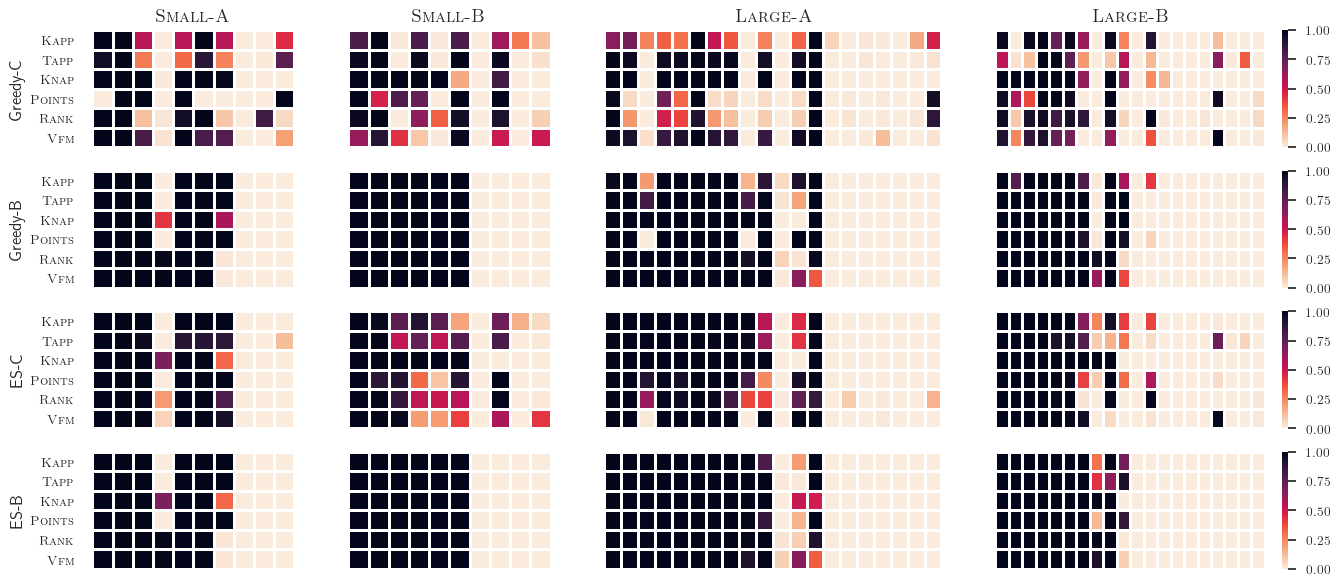
\includegraphics[width=15.5cm, height=7.5cm]{../experiment/heatmaps_all.png}
\caption{Stability heatmaps for  greedy aggregation (top) and \mes{} (bottom).
Within each panel each row represents an   input format and each column a project (ordered in increasing cost). The intensity of a cell indicates the fraction of instances in which the project was funded. 
}\label{fig:heatmap}
\end{center}\vspace{-3mm}
\end{figure*}

Strikingly, we see clear separation between binary and cost utilities. The outcome of the election is almost entirely unaffected by the choice of input format when using binary utilities --- the majority of the projects are either always funded under every input format or never under any.  
%Greedy aggregation exhibits this property only in rare instances, for example, the outcome of \textsc{Large-B} does not change if the input format is changed from \knap{} to \rank.  
This robustness to the choice of input format remains present when the number of sampled voters is varied $n'\in\{10,20,30\}.$
%
We also observe in   Figure~\ref{fig:heatmap} that aggregation with binary utilities is robust to partial participation: it is very rare that the decision to fund a project changes across repetitions when sampling voters at random, i.e.\ under a uniform model of voter participation/abstention. 
Cost utilities exhibit these properties only in rare instances.
%Greedy aggregation does not exhibit this property. 
 
While Figure~\ref{fig:heatmap} clearly establishes that binary utilities are more stable than cost utilities, it is less clear which aggregation method should be used when partial participation is a concern. \Cref{tab:ent_resp} reports the average entropy for each configuration. We observe that, no matter whether cost or binary utilities are used, \mes{} has lower entropy (and is thus more stable) than greedy aggregation.

\begin{table}[]
    \centering
    \caption{Average entropy and responsiveness as across configurations for the lab experiment. }
    \begin{tabular}{lcccc}
         \toprule
         &\multicolumn{2}{c}{Binary utility}& \multicolumn{2}{c}{Cost utility}  \\  \cmidrule(lr){2-3}\cmidrule(lr){4-5}
         & Greedy & \mes{} & Greedy & \mes{} \\
         \midrule
          Stability: entropy & 0.171 & 0.136 & 0.531 & 0.385 \\  
          Resposiveness: $n(V, A)$ & 0.252  & 0.280    & 0.115 & 0.217 \\
         \bottomrule
    \end{tabular}
    \label{tab:ent_resp}
\end{table}
% \begin{table}[htb]
%  \centering
% \begin{tabular}{llllll}
% \toprule
%                & 01-greedy & cost-greedy & 01-ES & cost-ES \\ \midrule
% entropy        & 0.171     & 0.531       & 0.136 & 0.385   \\ 
% \#swaps (in percentage) & 2.64      & 4.48        & 4.19  & 4.81    \\ \bottomrule
% \end{tabular}
% \end{table}\label{tab:ent_resp}

This experiment samples 40 votes from (on average) 58 consistent voters; as a result,  the sampled profiles are correlated and some degree of stability is expected. Next, we repeat the experiment, sampling $n'\in\{10,20,30\}$ voters each time, to investigate what happens when vote profiles are less correlated. 
%


Figure~\ref{fig:entropy} shows the entropy for election   \textsc{Large-B} across   input formats for aggregation methods when varying the degree of participation (i.e. the number of sampled voters). 
As expected, the correlation between vote profiles decreases and entropy increases  as fewer voters are sampled. 
As before, the entropy for binary utilities is consistently significantly lower than that of cost utilities across input formats. We conclude that binary utilities is significantly more robust to partial participation than cost utilities. One exception is worth highlighting, the entropy of cost utilities with \knap{} votes is fairly competitive with that of binary utilities. This suggests that if the organizers of a PB election are dead-set on using cost-utilities and also worried about the effect of partial participation,  \knap{} may be worth considering. 
%
For the other three elections,   binary utilities comfortably outperforms cost utilities across all input formats and sample sizes (except similar results for \knap{} in different elections). Full results  appear in the appendix. 

A final  interesting observation from  Figure~\ref{fig:heatmap} is unrelated to stability. It appears that expensive projects are  rarely funded  when using binary utilities, because it is very hard for  an expensive project to have a ratio of utility to cost that justifies funding it.

\begin{figure}[!h]
\begin{center}
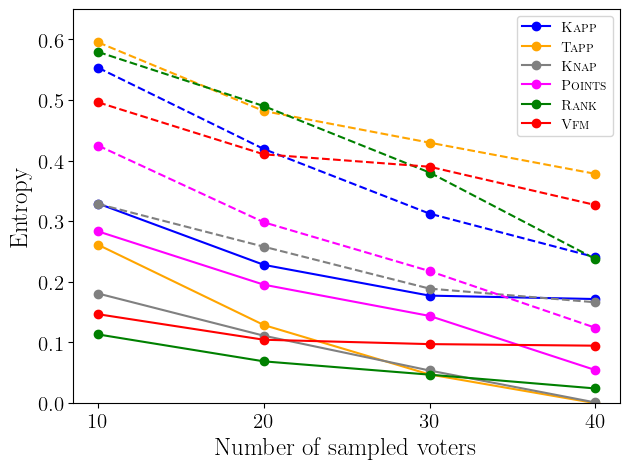
\includegraphics[width=7.5cm]{../experiment/entropy_greedy_large_b.png}
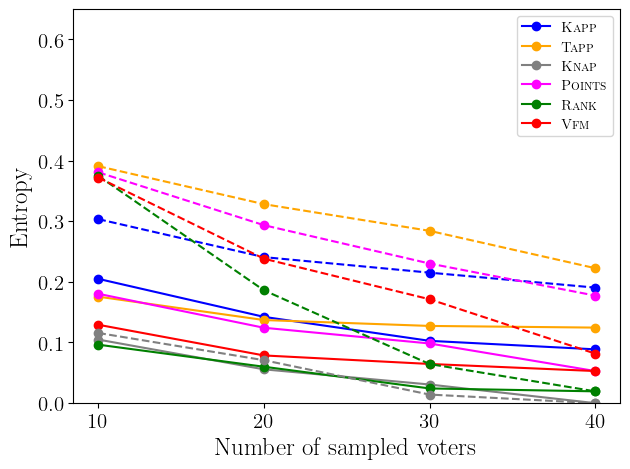
\includegraphics[width=7.5cm]{../experiment/entropy_es_large_b.png}
\caption{Entropy for each input format under  greedy aggregation  (left) and \mes{} (right)  as the degree of partial participation changes. Solid lines indicate binary utilities; dashed lines indicate cost utilities. 
}\label{fig:entropy}
\end{center}
\vspace{-3mm}
\end{figure}

%While it is clear using 01-utilities gives us better stability compared to cost-utilities, it not obvious whether greedy or \mes{} are better when using the same utilities. Table~\ref{tab:ent_resp} shows the average entropy we get from all instances. As can be seen the entropy lower if change between cost-utilities to 01-utilities and between greedy to \mes{}. Thus, indicating that on average \mes{} is more robust to partial participation than greedy.


\subsubsection{Responsiveness to campaigning}
We measure how responsive each election configuration is to campaigning by  determining how many (randomly selected) voters each voter must convince to change their vote before the outcome changes in their favor.
Figure~\ref{fig:responsiveness} show this average fraction of voters who need to be swayed to see an improved outcome. 

\costgreedy{} is  most responsive to campaigning, requiring less than 15\% of voters to be convinced before affecting the outcome regardless of the input format. 
We observe   that cost utilities lead to more responsive elections than binary utilities, and greedy aggregation is more responsive than \mes{}. The results are summarized in \Cref{tab:ent_resp} are consistent with these observations. 
%percentage of swaps required in order to improve the outcome for a voter. First we can see the amount of required swaps is relatively small (less than 10\% for all formats), this can be due to the small amount of voters or due to relatively high agreement on several projects thus "swaps" doesn't create big difference in the vote.

These results should be interpreted cautiously, since different aggregation methods yield different initial levels (and distributions) of social welfare, which may make it easier or harder to improve ones outcome. As an extreme example, consider an aggregation method which gives each voter their maximum possible utility: this aggregation method would, by our metric,  be entirely unresponsive simply because no voter can improve their outcome. 

\begin{figure}[htb]
\begin{center}
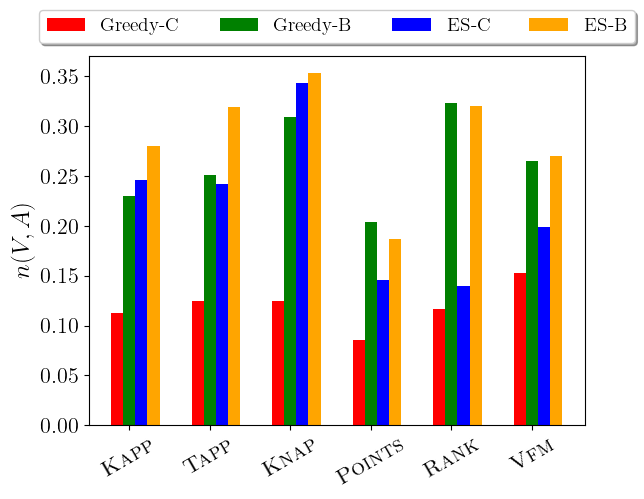
\includegraphics[width=7.5cm]{../experiment/avg_first_percentage.png}
\caption{Average percentage of voters that have to be convinced by campaigning to improve the outcome.  
}\label{fig:responsiveness}
\end{center}
\vspace{-3mm}
\end{figure}





%In contrast to the case of entropy, we see this time that the cost-utilities aggregation methods are more responsive compared to the 01-utilities aggregation methods. This make sense as cost-utilities focus on the amount of votes, while 01-utilities focus on the ratio between utility and cost. In addition, we see in most cases that the greedy aggregation is more responsive compared to ES. This can also be seen in Table~\ref{tab:ent_resp} where the average percentage of required swaps is shown for each aggregation method.

% \subsection{Social Welfare}
% An obstacle to comparing outcomes based on social welfare is participants are assigned only one format, so there is no common basis of comparison when aggregating vote profiles from different formats. To address this, we make the assumption that, since voters are randomly assigned to input formats, the distribution of voter preferences are the same across formats. As such, we can deduce voter valuation functions from the full vote profile in \emph{any} format and treat these aggregated values as a proxy for the welfare of all voters, regardless which format they used.\footnote{ We caution that this is at best a very coarse evaluation, since assuming a value based on  a vote in any of the formats requires very strong assumptions. 
% } 

% We report in Figure~\ref{fig:welfare} the   social welfare (averaged over the four elections) as measured when treating the full profile of \points{} or \knap{} voters as representative. 

% Neither aggregation method strictly outperforms the other. However, we observe that, when using greedy aggregation, the choice of input format can have a large effect on welfare. This is seen most clearly when using \knap-voters to compute welfare. Unsurprisingly, \mes{} is less sensitive to  the choice of input format and   achieves very similar welfare across input formats.
% Results when using the other formats to measure welfare are less extreme than the results shown here and may be found in the full version.

% \gb{discuss responsiveness here once we have the figure. depending on clarity, figure may go to appendix}

\section{Evidence from real participatory budgeting elections}\label{sec:real}
% Pabulib instances
% \begin{itemize}
%     \item Overall plots, comparison with 4 lines. scatter plots with 
%     \item Plot with size on x axis - which instances
% \end{itemize}  

We extend our study of aggregation methods to the participatory budgeting instances available on a public repository called \pabu{} \citep{pabulib}. \pabu{} consists of the votes cast in more than 700 participatory budgeting elections held across Poland. 
These real-world elections are much larger than those in our lab experiment, the largest elections have more than $100\,000$ voters and more than 100 projects.
In contrast to our experiments, voters in real elections cast a vote in only one format; we focus our analysis on elections reporting approval votes between 2015 and 2023, of which there are  532 at the time of analysis. The characteristics of these elections are summarized in \ref{tab:pabulib}. %\footnote{Correct to the time of writing the paper}. 

\begin{table}[htb]
    \centering
    \caption{Summary of the 532 \pabu{} instances analysed. }
    \label{tab:pabulib}
    \begin{tabular}{lcccc}
    \toprule
         Voters  & $<1$k & $1-10$k & $>10$k & Total   \\ \midrule
        Elections & 157 & 330 & 45 & 532\\
        %Avg. number of  projects & 8.75  & 28.60 &  76.35 & 26.78 \\
        Avg. number of  projects & 8.8  & 28.6 &  76.4 & 26.8 \\
        Avg. budget    & 383k & 124k & 7\,810k & 1\,543k\\
        Avg. project cost   & 86k & 209k & 643k & 210k \\\bottomrule
    \end{tabular}
    
\end{table}

\subsection{Welfare and representation}

We start by calculating the welfare and representation achieved by each of the aggregation methods for all instances. Figure~\ref{fig:wel_rep_pab} plots the average social welfare across the 532 elections against the average representation score, as measured by $R(F)$ for outcomes $F$. 
\costgreedy{} leads to significantly lower social welfare than the alternative configurations ($p<0.05$), while both ES variants lead to significantly lower representation than their greedy counterparts. It is somewhat surprising that, though ES guarantees a form of proportionality, we observe less representative outcomes than under greedy aggregation (which provides no proportionality guarantees). %\gb{Roy: please confirm both ES worse than both greedy ito representation?} \rf{It is indeed the case.}
%show the average welfare Vs average representation for each of the methods. We see that cost-greedy achieve significantly ($p<0.05$) worse welfare compared to other methods and 01-ES achieve significantly worse representation from the greedy methods. Interestingly, while ES guarantee proportional outcome, it work worse than greedy in terms of representation.

\begin{figure}[!h]
\begin{center}
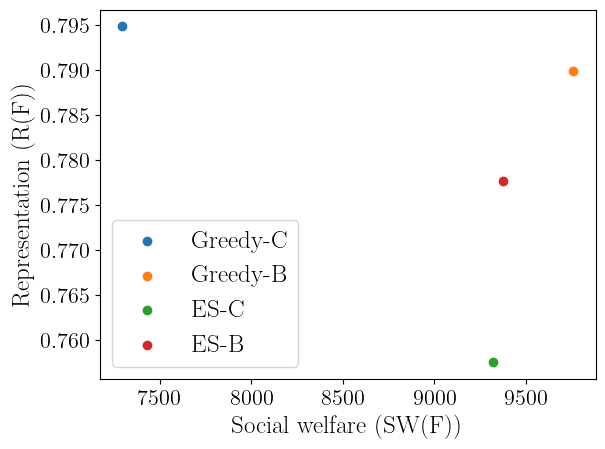
\includegraphics[width=7.5cm]{../experiment/avg_scores.png}
\caption{Average social  welfare ($\sw(F)$) plotted against   representation ($R(F)$) across 532 \pabu{} instances. 
}\label{fig:wel_rep_pab}
\end{center}
\vspace{-3mm}
\end{figure}

\subsection{Stability to partial participation}


% Of these, we omit xxx due to ....\gb{Roy   please check all these numbers to make sure we report what we actually did. }\rf{It seems that they updated pabulib, there are currently 532 instances. I ran on 469 (because this what existed when I downloaded it). I will download the latest data and create again the graph. We don't omit any of them, only filter by amount of projects (As in figure 10)}

We run a   similar experiment to before, sample an $n'$ fraction of voters from each election and aggregate these votes  using greedy aggregation and \mes, assuming both binary and cost utilities. This is repeated 2000 times, we report averaged results in \Cref{fig:pabulib:stability} for $n'\in \{0.01, 0.03, \ldots, 0.11\}$.\footnote{Constraints on computation time are the only obstacle to further experiments: the experiment for $n' = 0.11$ takes several days to complete.%\rf{I didn't save the runtime} \gb{would be nice to have  a reason why we didn't test larger - do you have a rough estimate?}\rf{Running up to this number took several days}
}

\begin{figure}[!h]
\begin{center}
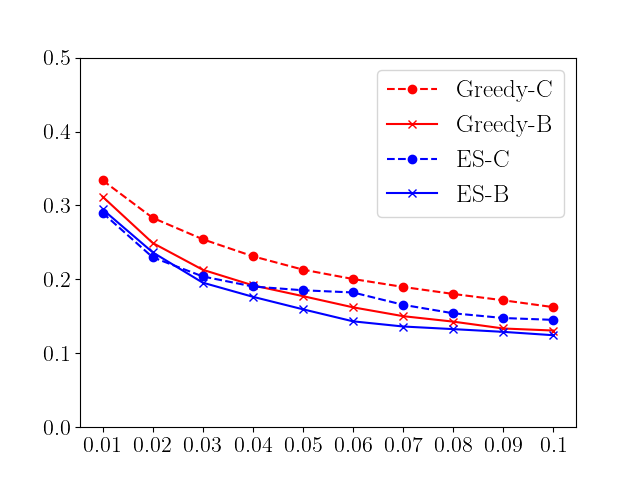
\includegraphics[width=7cm]{../experiment/entropy_pabu_small.png}
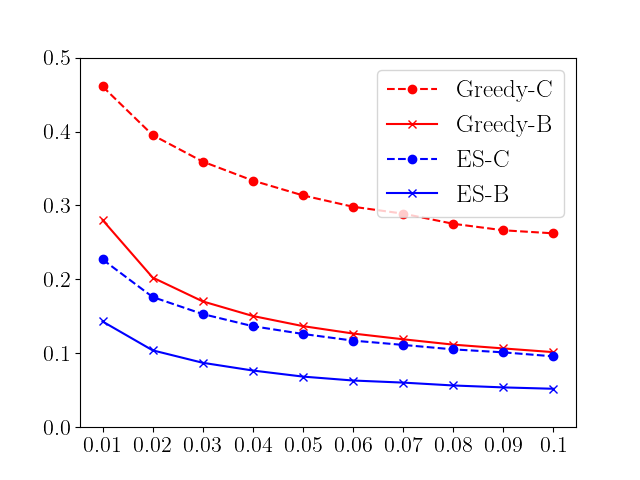
\includegraphics[width=7cm]{../experiment/entropy_pabu_large.png}
\caption{Entropy for each input format  and aggregation rule under binary and cost utilities. Results for small elections with at most 10  projects on the left, larger elections on the right. 
}\label{fig:pabulib:stability}
\end{center}
\vspace{-3mm}
\end{figure}

We analyze small elections with at most 10 projects separately from larger elections. 
Small elections provide little flexibility in which projects to fund, as a result we notice very similar stability across configurations. 
On larger elections, however,  we observe as before that \mes{} is considerably more stable than greedy aggregation (regardless of the utilities used) and the outcomes are more stable when using binary utilities than for cost utilities. 


Digging deeper into what exactly causes the difference in stability   between small and large elections, we define the difference in entropies 
\[
\Delta(A) = \text{entropy}^{\mes}( A) -  \text{entropy}^{Greedy}( A)
\]
on instance $A$.\footnote{All   \pabu{} instances we analyze consist of approval votes, so we suppress the dependence on $V$, the voting format.} 
Let $B_A$ and $\bar{c}_A$ be the budget and average cost of a project in instance $A$. 
\Cref{fig:pabulib:entvsbudget} plots  $\Delta(A)$ against the expected number of projects funded, $n_A \triangleq B_A / \bar{c}_A$ for the  \pabu{} instances with at least 10 projects, assuming 1\% participation.
\bingreedy{} has higher entropy than \mes{} almost exclusively on those instances where the budget and project costs are such that at most two projects can be funded. On instance with more flexibility and a larger number of feasible outcomes, \mes{}  is consistently more stable. These findings hold when varying the utility model (see \Cref{fig:pabulib:entvsbudget}, right) and the fraction of votes sampled (refer to the appendix). 


\begin{figure}[!h]
\begin{center}
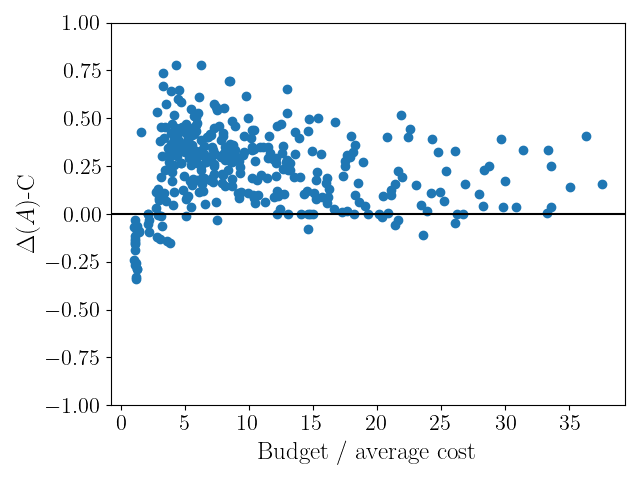
\includegraphics[width=7cm]{../experiment/greedy_ES_cost_0.01.png}
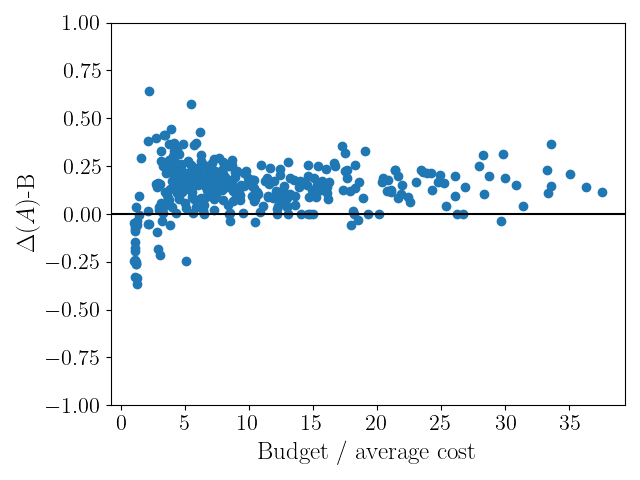
\includegraphics[width=7cm]{../experiment/density_greedy_ES_0.01.png}
\caption{Regardless of the utility model used (cost: left, binary:right), \mes{} is consistently more stable than greedy on non-trivial elections. 
%Difference in entropy between \mes{} and greedy at 10\% participation versus the average number of projects funded across large instances for cost-utilities (left) and 01-utilities (right).   
}\label{fig:pabulib:entvsbudget}
\end{center}
\vspace{-3mm}
\end{figure}

\subsection{Responsiveness to campaigning} 
We repeat our responsiveness analysis on \pabu{} elections. We omit 16.8\% of the elections on the basis that all voters already receive their maximum possible utility, so there is no reason to or benefit from campaigning. 



 Figure~\ref{fig:pabulib:unchanged} reports the average percentage of voters who receive maximal welfare in the original  outcome (before any campaigning). These voters can not improve their outcome from campaigning, so we omit them from the experiment. 
 Unsurprisingly \costgreedy{} has significantly more such saturated voters than alternative configurations ($p < 0.05$). We speculate that this is a result of greedy fully satisfying majority groups who support budget feasible  sets. \mes{}, on the other hand, provides some proportionality guarantees which may leave majorities with some room for improvement. % suggest that the minimum welfare is likely higher this due the fact it choose the projects with the highest support increasing the chance to satisfy the biggest amount of voters. ES on the other hand focus on proportionality i.e., focusing on giving sufficient representation to the voters, thus it can make more people well represented, but leaving more room for improvement.
  

Figure~\ref{fig:pabulib:resp} shows the average fraction of the population that a campaign must reach before increasing the campaigners welfare (for those voters who don't already receive maximal welfare). Elections using \mes{} are consistently less responsive to campaigning than those using greedy aggregation.  These results align with our expectations  described in Section~\ref{sec:pred}.

It is possible that \mes{} is less responsive to campaigning because voters start out receiving higher utilities, making it harder to increase their utility through campaigning. In Figure~\ref{fig:wel_improve} we report the average welfare of those voters who are able to benefit from campaigning, as well as the average improvement  that they see after campaigning. Interestingly, \costgreedy{} starts with the lowest average welfare despite having the most voters with maximal utility. This supports the narrative that \costgreedy{} saturates a majority at the cost of giving remaining voters very low welfare. This, in turn, yields a large fraction of the population that are able to see significant gains from campaigning. There is little to distinguish between other methods. 


%To complete the picture, Figure~\ref{fig:wel_improve} show the average welfare a voter receive from each aggregation method before and after "convincing" other voters to change their votes. The figure shows that cost-greedy starts with the lowest average welfare, this can be explained by the large amount of voters that reach their maximal welfare compare to the other aggregation methods as seen in Figure~\ref{fig:pabulib:unchanged}. In this method very popular projects will be selected, leaving many voters who prefer less popular projects under-represented, resulting with lower satisfaction on average and leaving more room for improvement. For the other methods we see that they all start and end with similar average welfare.

 

\begin{figure}[!h]
\begin{center}
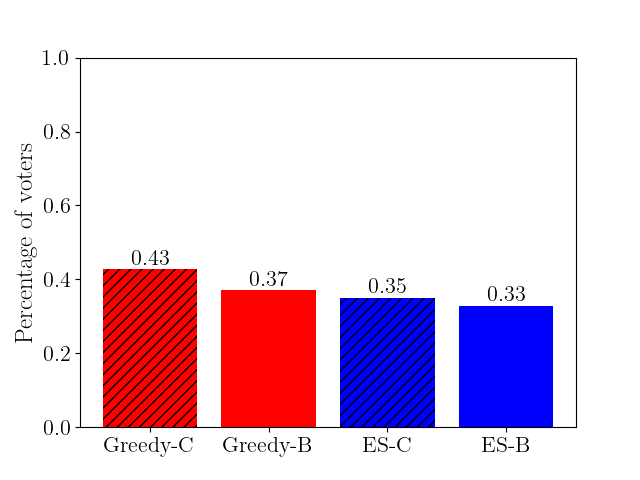
\includegraphics[width=7cm]{../experiment/unchanged_percent.png}
\caption{Fraction of voters that receive their maximal welfare before campaigning. %Red for Greedy and stripes for cost utilties.
}\label{fig:pabulib:unchanged}
\end{center}
\vspace{-3mm}
\end{figure}

\begin{figure}[!h]
\begin{center}
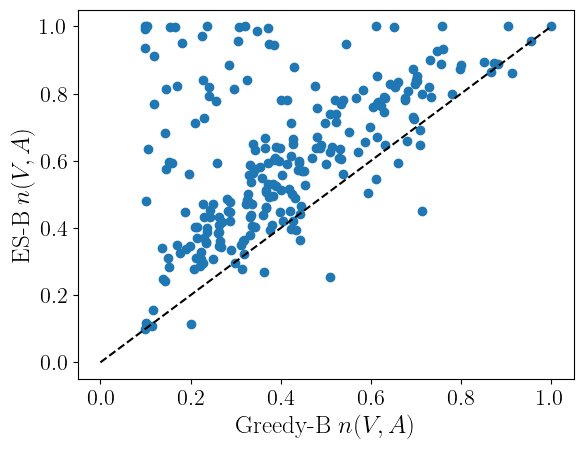
\includegraphics[width=7cm]{../experiment/resp_01.png}
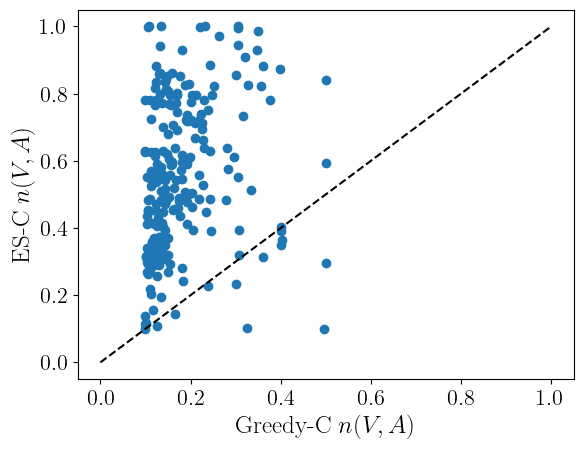
\includegraphics[width=7cm]{../experiment/resp_cost.png}
\caption{$n(V, A)$ for greedy VS \mes{} under binary (left) and cost utilities (right). 
%\gb{Should the x and y axis both refer to $n(V,A)$ here?}
}\label{fig:pabulib:resp}
\end{center}
\vspace{-3mm}
\end{figure}

\begin{figure}[!h]
\begin{center}
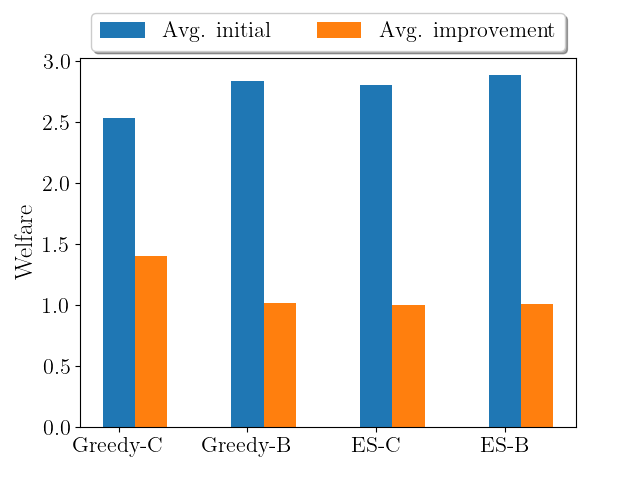
\includegraphics[width=7.5cm]{../experiment/welfare_improvement.png}
\caption{Average voter welfare before campaigning and improvement from campaigning. 
%\gb{y-label:Welfare. move legend so that it isn't in the way (perhaps bottom or outside). legend labels: if y-axis is welfare, the legend labels can be as short as 'avg. initial', 'avg. improvement'. If you want to use longer  we don't really use the 'swaps' terminology in the paper, so perhaps make it 'avg. improvement from campaigning'. }
}\label{fig:wel_improve}
\end{center}
\vspace{-3mm}
\end{figure}

In conclusion, Table~\ref{tab:pabu_ent_resp} summarizes the stability and responsiveness on \pabu{} instances. These results are consistent  with the findings of our lab experiment: binary utilities are more stable than cost utilities and \mes{} is more stable than greedy aggregation. \gb{the way es beats greedy is not the same as the way binary beats cost.}
However, this comes at the cost of responsiveness, \mes{} (binary utilities) is less responsive to campaigning than greedy aggregation (cost utilities). 
%To conclude the section, Table~\ref{tab:pabu_ent_resp} shows the average entropy and number of swaps for \pabu{} instances. We can see that by using 01-utilities instead of cost-utilities and \mes{} instead of greedy results in outcomes that are more stable to partial participation. However, this come with a cost, while those rules are more stable, they are also less responsive. Therefore, it require to convince more voters to change their vote in order to make an effect in the outcome in favor of specific voter.

\begin{table}[htb]
    \centering
    \caption{Average entropy and responsiveness on \pabu{} elections. }
    \begin{tabular}{lcccc}
         \toprule
         &\multicolumn{2}{c}{Binary utility}& \multicolumn{2}{c}{Cost utility}  \\  \cmidrule(lr){2-3}\cmidrule(lr){4-5}
         & Greedy & \mes{} & Greedy & \mes{} \\
         \midrule
          Stability: entropy & 0.290 & 0.192 & 0.419 & 0.247 \\  
          Resposiveness: $n(V, A)$ & 0.41  & 0.61    &  0.177 &  0.543 \\
         \bottomrule
    \end{tabular}
    \label{tab:pabu_ent_resp}
\end{table}

% \begin{table}[]
% \rf{Possibly replacing the table with a figure.}
% \centering
% \begin{tabular}{|l|l|l|l|l|}
% \hline
%                & 01-greedy & cost-greedy & 01-ES & cost-ES \\ \hline
% entropy        & 0.290     & 0.419       & 0.192 & 0.247   \\ \hline
% \#swaps (in percentage) & 41.2      & 17.7        & 61.3  & 54.3    \\ \hline
% \end{tabular}
% \end{table}\label{tab:pabu_ent_resp}



\section{Discussion} 
 

These results highlight practical insights  for the design of real participatory budgeting elections. 
When choosing an input format, we find no reason to deviate from the current standard practice of  using \kapp{} voting: Voters find the format easy to understand, easy to  use, and believe it allows them to express their preferences accurately. 

Greedy aggregation is used almost universally,  however, our experiments find that \mes{} has  two  big advantages over greedy aggregation.  First,  the outcomes are largely stable and unchanged when only a subset of the population participates. In light of low levels of real-world participation, we believe this is a particularly attractive property. Second, \mes{} appears to be robust to the choice of input format, in other words, it affords the city officials responsible for administering the participatory budgeting election a great deal of freedom to choose an input format which meets whatever secondary objectives are deemed to be important. % means that it allows officials a large degree of freedom to choose an input format which suits their objectives

We find find the argument for stability (extremely low real-world turnout) compelling, but it is certainly not the last word. An argument against stability is that an aggregation rule should be responsive;  the outcome of an election \emph{should} change when the preferences of the voters change.  An example of a well-publicized electoral process which is not responsive is gerrymandered congressional districts in the US, where voters are grouped in such a way that the elected representatives have are largely unaffected by swings in partisan support. This may lead to voters feeling disenfranchised .
However, an election being responsive to campaigning is somewhat of a double-edged sword: it also allows wealthy entities to influence the election outcome towards their preferences. 
Though there is no definitive answer as to what level of responsiveness to campaigning is ideal, we do believe that this is something which the organizers of participatory budgeting elections should keep in mind. 
We find that elections using greedy aggregation are  typically more responsive  than those using \mes, and generally find stability to be inversely correlated with  responsiveness.
%Towards this line of thought we report in the appendix  on experiments aimed at responsiveness: we measure how many copies of each voter is required (how many similar voters they must recruit) to improve their utility from the funded set of projects. 


%Finally, a negative correlation was observed between stability and responsiveness. The selection of a particular method by the designer depends on whether they aim to encourage voters to adopt a more strategic approach or not. When employing a more responsive method, individuals are incentivized to invest effort in persuading others about their preferred projects to secure votes. Conversely, with less responsive rules, individuals may perceive the benefits of exerting effort to convince others as not worthwhile. Hence, in terms of responsiveness, there is no definitive answer, but rather a factor to be deliberated upon when organizing participatory budgeting to align with specific objectives.

%One argument that remains in favour of greedy aggregation is its transparency: it is arguably easier to explain to voters than \mes{}. If greedy aggregation is used    and stability to partial participation is a primary concern, then \knap{} emerges as a fairly user-friendly format overall and a clear front-runner in terms of stability.


%\gb{Robustness as argument against stability. appendix. also social welfare - appendix. }
The findings of our user study  are consistent across several election sizes and input formats, and align with the results from more than 500 real participatory budgeting elections in Poland. Still, we highlight some limitation of the study. The  behavior and preferences of participants recruited on Amazon Mechanical Turk likely do not perfectly match those of real voters and it is possible that, despite our best efforts, the   voter experience   was affected by the interface design choices we made.   PB elections overwhelmingly use $k$-approval votes, we are unable to provide real-life evidence for the alternative voting formats. 

% These recommendations should be taken in the context of the limitations of this study. First, the  behavior and preferences of participants recruited on Amazon Mechanical Turk may not be sufficiently similar to those of real voters.  Though we attempt to  ensure the findings are robust across the parameters of different elections by varying the number and type of projects, there is no mimicking the richness, variety and local idiosyncrasies of real-world instances. Similarly, real voter utilities likely exhibit complementarities and externalities  --- a far cry from our utility proxies. It is possible that, despite our best efforts, the   voter experience   was affected by the interface design choices we made. 

% We find find the argument for stability (extremely low real-world turnout) compelling, but it is certainly not the last word. An argument against stability is that an aggregation rule should be responsive;  the outcome of an election \emph{should} change when the preferences of the voters change.  An example of a well-publicized electoral process which is not responsive is gerrymandered congressional districts in the US, where voters are grouped in such a way that the elected representatives have are largely unaffected by swings in partisan support. Towards this line of thought we report in the appendix  on experiments aimed at responsiveness: we measure how many copies of each voter is required (how many similar voters they must recruit) to improve their utility from the funded set of projects. 
% This measure of responsiveness is largely inverse to stability but not strictly so, for example, with binary utilities \mes{} is both more responsive and more stable than greedy aggregation. 

We conclude with  two directions for future study.  
When it comes to designing participatory budgeting elections, the proof, to a large extent, should be in the pudding.   
One can imagine a  variant of the experiment presented in this paper in which votes from different PB designs are aggregated and voters are directly asked to compare different elections and outcomes on the transparency of the process, personal satisfaction, perceived fairness of the outcome, etc. 
Directly asking people their opinion about PB outcomes may yield new  insights   that can help inform design decisions while avoiding assumptions like  additive utilities. 

Democratic innovations live and die by the extent to which voters' voices are heard. But this requires representative participation. 
As a fledgling part of the democratic process, participatory budgeting appears to be particularly susceptible to poor participation. It is important to understand how   design choices around voting formats and the transparency of aggregation rules affects the participation (now and in the future) of voters from a wide range of socio-economic backgrounds. Our stability experiments are a step in this direction but assume participation is uniform across the population, which is unlikely to reflect reality. 

\gb{Roy: there are several issues in the bibliography. Inconsistent abbreviation of author names. missing capital letters (stewart et al, Su), inconsistent capitalisation of paper titles and journal names. etc.}
\bibliography{ref}
\bibliographystyle{plainnat}


\end{document}
